\documentclass[a4paper,11pt,twoside]{article}
\usepackage{makeidx}
\usepackage{amsfonts}
\usepackage{fullpage}
\usepackage{amsmath}
\usepackage{amssymb}
\usepackage{amsthm}
\usepackage{appendix}
\usepackage{graphicx}  
\usepackage{manfnt}
\usepackage{marginnote}
\usepackage{xfrac}
\usepackage{xcolor}
\usepackage{framed}
\usepackage{hyperref}
\newtheorem{thm}{Theorem}[subsection]
\newtheorem{lem}[thm]{Lemma}
\newtheorem{prop}[thm]{Proposition}
\newtheorem{cor}[thm]{Corollary}
\newtheorem*{signals}{Signal}
\newtheorem*{appdom}{Application domain}
\theoremstyle{definition}
\newtheorem{ex}[thm]{Example}
\newtheorem{defn}[thm]{Definition}
\newtheorem{cont}[thm]{Conjecture}
\theoremstyle{remark}
\newtheorem{rmk}[thm]{Remark}
\newtheorem{addendum}[thm]{Addendum}
\usepackage{theoremref}
\usepackage[all]{xy}
\usepackage{mathrsfs}
\usepackage{listings}
\usepackage{xcolor}
\usepackage{tikz}
\usetikzlibrary{arrows}
\newcommand{\x}{\mathrm{x}}
\newcommand{\y}{\mathrm{y}}
\newcommand{\z}{\mathrm{z}}
\newcommand{\JSD}{\mathrm{JSD}}
\newcommand{\mean}{\mathrm{mean}}
\newcommand{\sh}[1]{\colorbox{pink}{#1}}
\newcommand{\lnk}[1]{\sh{\hyperref[#1]{\ref*{#1}}}}

\newenvironment{sigs}
   {\colorlet{shadecolor}{green!50}\begin{shaded}\begin{signals}}
   {\end{signals}\end{shaded}}

\newenvironment{app}
   {\colorlet{shadecolor}{red!50}\begin{shaded}\begin{appdom}}
   {\end{appdom}\end{shaded}}

\newcommand{\bad}[1]{\colorbox{orange}{#1}}

\begin{document}
\title{\textbf{Signals for Point Clouds}}
\author{\copyright\ Data Signals Ltd No 3 Hardman Square Manchester M3 3EB, \underline{UK}
}
\date{}
\maketitle
\includegraphics[width=1\textwidth]{manchester.png}
\newpage
\tableofcontents
\lstset{language=Python, 
        basicstyle=\ttfamily\small, 
        breaklines = true
}
\newpage
\section{Signals} 
\subsection{Making signals}
Points in a point cloud possess basic attributes. These may include, and may not be limited to:
\begin{itemize}
\item A position $(x,y,z)$ in 3D space. (Three 32-bit integers when unscaled, or three 64-bit floats when scaled.)
\item An intensity. (An unsigned 16-bit integer.)
\item Return number and number of returns. (An unsigned 8-bit integer.)
\item Classification. (Unsigned 8-bit integers.)
\item Time. (A 64-bit float.)
\end{itemize}
For now, a \textbf{signal} is an attribute of the points in the point cloud which may be derived from the basic attributes. These attributes will be positive real numbers, and we will plot them by storing their values as the intensity of points in a LAS file. If a point cannot have such an attribute assigned to it for any particular reason, we could exclude it from the signal. Often our signals will be given by geometric statistics, but they may also be given by the selection of a family of points in the point cloud which have a special property, i.e. they may be boolean-valued signals. If our signals are boolean, then we will plot the signals as raw classification rather than as intensity.

\begin{rmk}Some of our signals are given by regression coefficients. These statistics only attain values between 0 and 1, so it's important to remain aware of the caveat that if we store these raw numbers as intensities (i.e. 16-bit integers), they will be set to either $0$ or $1$. Therefore, we will multiply these signals by 1000 before plotting them. When we colour our point clouds in Displaz, we will divide by 1000 again to get a number between 0 and 1, which will allow us to represent a colour in Displaz.
\end{rmk}
Suppose we have a collection of 3-vectors
\begin{displaymath}
\{\textbf{r}_0=(x_0,y_0,z_0),\textbf{r}_1=(x_1,y_1,z_1),\textbf{r}_2=(x_2,y_2,z_2),\dots,\textbf{r}_{n-1}=(x_{n-1},y_{n-1},z_{n-1})\}
\end{displaymath}
which constists of positions in the point cloud. 
\begin{sigs}
The \textbf{covariance} of vectors $(x_0,x_1,x_2,\dots,x_{n-1})$ and $(y_0,y_1,y_2,\dots,y_{n-1})$ is given by
\begin{displaymath}
c_\mathrm{xy}=\frac{1}{n}\sum_i(x_i-\overline x)(y_i-\overline y),
\end{displaymath}
where $\overline x$ and $\overline y$ are the \textbf{means}, given by
\begin{align*}
\overline x&=\frac{1}{n}\sum_i x_i
\\
\overline y&=\frac{1}{n}\sum_i y_i.
\end{align*}
\end{sigs}
We could also take yz-covariance and zx-covariance. So, we get the covariances
\begin{displaymath}
c_\mathrm{xy}\text{, }c_\mathrm{yz}\text{, }c_\mathrm{zy}
\end{displaymath}
and standard deviations, 
\begin{displaymath}
\sigma_\mathrm{x}=c_\mathrm{xx}^{1/2}\text{, }\sigma_\mathrm{y}=c_\mathrm{yy}^{1/2}\text{, }\sigma_\mathrm{z}=c_\mathrm{zz}^{1/2}.
\end{displaymath}

Many of the signals herein are built out of statistics such as these. But we can't rightly call a single statistic a ``signal". We'll instead take statistics at a local scale. Many of our signals will have parameters:
\begin{itemize}
\item a \textbf{radius} $\epsilon>0$,
\item a \textbf{k-number} $k>0$, $k\in\mathbb{Z}$.
\end{itemize}

(There are more parameters to follow, but their purpose takes more explaining.)

Given any statistic which makes sense for a family of 3-vectors, we can build a function $f$ by using the following recipe to evaluate $f(\textbf{r})$ at any point $\textbf{r}=(x,y,z)$:
\begin{itemize}
\item Find the $k$ points in the point cloud that are nearest to the position $\textbf{r}$, with positions $\textbf{r}_0,\textbf{r}_1,\dots,\textbf{r}_{k-1}$. (Including $\textbf{r}_0=\textbf{r}$ itself, if a point has position $\textbf{r}$.)
\item Discard the points $\textbf{r}_i$ such that $\lVert \textbf{r}-\textbf{r}_i\rVert\geqslant\epsilon$.
\item Take the statistic for the remaining points, and let this be the value $f(\textbf{r})$.
\end{itemize}
This function becomes a signal, because we can take it as a new attribute for any point in our point cloud. If a point has position $\textbf{p}$ and has enough near neighbours, it now obtains the new attribute $f(\textbf{p})$. Signals derived like this are ``geometric signals" because they only require the 3-vectors which give the positions of our points in order to be computed.

Therefore, for any point cloud, we obtain covariance attributes $c_{\x\y}(\textbf p)$, $c_{\y\z}(\textbf p)$, $c_{\z\y}(\textbf p)$ and standard deviation functions $\sigma_\x(\textbf p)$, $\sigma_\y(\textbf p)$, and $\sigma_\z(\textbf p)$. Consequently, we obtain the corresponding signals.

\begin{rmk}The reasons we insist on the parameters, $\epsilon$, $k$, are the following.
\begin{itemize}
\item Keeping our points within a sphere of radius $\epsilon$ stops our $k$ nearest neighbours from being so far apart that we cannot rely on the result. If two object types are sat close together in the landscape, e.g. two cars, then the nearest neighbours of points on one object may be actually from the other object. We want to avoid the mixing of objects.
\item Varying $k$ allows us to increase the quality of our signals which measure the relationship between near neighbours.  Putting an upper bound on the number of neighbours keeps the number of calculations from growing out of control.
\end{itemize}
\end{rmk}
\begin{addendum}\label{add}One of the problems in lidar data is oversampling caused by the aircraft slowing down or rotating, thus causing some points to have far more neighbours than other points. This is indicated by the space-time diagram (with elevation set to time) in Figures \hyperref[spacetime]{\ref*{spacetime}}, \hyperref[spacetime]{\ref*{spacetime1}}. We'll fix this problem later, but it will require us to introduce a new parameter to some signals.
\end{addendum}
\newpage
\begin{figure}[!h]
  \caption{Space-time diagram of conductor}
  \centering
    \includegraphics[width=0.9\textwidth]{spacetime.png}
    \label{spacetime}
    \newline{Space-time bending back on itself corresponds to turning point in attitude of aircraft}
\end{figure}
\begin{figure}[!h]
  \caption{Space-time diagram of vegetation}
  \centering
    \includegraphics[width=0.9\textwidth]{spacetime1.png}
    \label{spacetime1}
    \newline{Oversampling is caused at the ``folds"}
\end{figure}
\newpage
\subsection{Covariance signals}
Suppose we have a family of points $\{(x_i,y_i,z_i):i = 0,1,,2\dots, n-1\}$. 
\begin{sigs}
The \textbf{covariance matrix} is given by
\begin{displaymath}
C = \begin{pmatrix}
\sigma_{\x}^2 & c_{\x\y}&c_{\x\z}\\
c_{\y\x}&\sigma_\y^2&c_{\y\z}\\
c_{\z\x}&c_{\z\y}&\sigma_\z^2
\end{pmatrix}.
\end{displaymath}
\end{sigs}
\begin{app}The covariance matrix is an operator which encodes the shape of a family of points. We will see how the nature of the shape can be deduced.
\end{app}
Since the covariance matrix is symmetric, it is orthogonally diagonalisable -- so says the Spectral Theorem \cite[Theorem 5.20]{poole}. 

For any vector 
\begin{displaymath}
\mathbf{v} = \begin{pmatrix}a\\b\\c
\end{pmatrix}
\end{displaymath}
we have
\begin{displaymath}
\mathbf{v}^TC\mathbf{v}=\overline w
\end{displaymath}
where $\overline w=\frac{1}{n}\sum^n_{i=1}w_i$ is the mean of the derived attribute
\begin{displaymath}
w_i = (a(x_i-\overline x)+b(y_i-\overline y)+c(z_i-\overline z))^2.
\end{displaymath}
of our points\footnote{To prove this, note that $C=AA^T$ where $A$ is the $3\times n$ matrix
\begin{displaymath}
\frac{1}{\sqrt{n}}\begin{pmatrix}
x_0&x_1&\dots & x_{n-1}\\
y_0&y_1&\dots & y_{n-1}\\
z_0&z_1&\dots & z_{n-1}
\end{pmatrix},
\end{displaymath}
and, therefore, $\textbf{v}^TC\textbf{v}=\textbf{v}^TAA^T\textbf{v}=(a^T\textbf{v})^T(A^T\textbf{v})=\lVert A\textbf{v}\rVert ^2=\overline w$.}. Now, the points $(x_i,y_i,z_i)$ are coplanar if and only if $w_1=w_2=\dots=w_n=0$, or equivalently $\overline w=0$, for some vector $\mathbf{v}\neq \mathbf{0}$.

Since $C$ is orthogonally diagonialisable, there is an orthonormal basis $\{\mathbf{v}_0,\mathbf{v}_1,\mathbf{v}_2\}$ of $\mathbb{R}^3$ which consists of eigenvectors of $C$. Let $\{\lambda_0,\lambda_1,\lambda_2\}$ be the correpsonding eigenvalues. If $\mathbf{v}=a_0\mathbf{v}_0+a_1\mathbf{v}_1+a_2\mathbf{v}_2$ then the corresponding attribute $w$ is such that 
\begin{displaymath}
\overline w = \mathbf{v}^TC\mathbf{v}= a_0^2\lambda_0+a_1^2\lambda_1+a^2_2\lambda_2.
\end{displaymath}
Since $C$ generates a non-negative bilinear form (because we always have $\overline w\geqslant 0$), $\lambda_0,\lambda_1,\lambda_2\geqslant 0$. The points $(x_i,y_i,z_i)$ are coplanar if and only if the matrix $C$ is \emph{not} positive definite, i.e. if $\det C =\lambda_0\lambda_1\lambda_2 =0$.

This matrix is the parent to many signals which we can plot:
\begin{itemize}
\item \hyperref[lab0]{\sh{Planar regression.}}
\item \hyperref[lab1]{\sh{XY-linear regression.}}
\item \hyperref[lab2]{\sh{3D linear regression.}}
\item \hyperref[lab3]{\sh{Ruggedness.}}
\item \hyperref[evalz]{\sh{Eigenvalues and rank.}}
\end{itemize}
We will order the eigenvalues so that $\lambda_2\geqslant \lambda_1\geqslant\lambda_0\geqslant 0$. The eigenvalues determine the behaviour of the points according to the following table.
\begin{center}
\begin{tabular}{| c|c|c }
 Eigenvalues close to 0 & Behaviour  \\\hline 
  None & Points spread out \\
 $\lambda_0$, not $\lambda_1$& Coplanar, not colinear\\ 
 $\lambda_0$, $\lambda_1$, not $\lambda_2$ & Colinear, not concentrated around a point \\  
 $\lambda_0$, $\lambda_1$, $\lambda_2$ & Concentrated around a point
\end{tabular}
\end{center}
We will prove that this table is right in Section \hyperref[evals]{\ref*{evalz}}.
\newpage
\subsubsection{Planar regression}\label{lab0}
We would like a measure for the coplanarity of our points. We will derive this measure from the coplanarity matrix $C$ which we have already met.

Now, since $C$ is a non-negative matrix,
\begin{displaymath}
\det C = (\sigma_\x^2\sigma_\y^2\sigma_\z^2+2c_{\x\y}c_{\y\z}c_{\z\x})-(\sigma_\x^2c_{\y\z}^2+\sigma_\y^2c_{\x\z}^2+\sigma_\z^2c_{\x\y}^2)\geqslant 0
\end{displaymath}
so 
\begin{displaymath}
\frac{\sigma_\x^2c_{\y\z}^2+\sigma_\y^2c_{\x\z}^2+\sigma_\z^2c_{\x\y}^2}{\sigma_\x^2\sigma_\y^2\sigma_\z^2+2c_{\x\y}c_{\y\z}c_{\z\x}}\leqslant 1
\end{displaymath}
with equality if and only if the points $(x_i,y_i,z_i)$ are coplanar. Note that if the denominator is zero, so is the numerator, and this ensures that the points are coplanar anyway.
\begin{sigs}
We define the statistic
\begin{displaymath}
p_{\x\y\z}=\begin{cases}1&\sigma_\x^2\sigma_\y^2\sigma_\z^2+2c_{\x\y}c_{\y\z}c_{\z\x}=0\\
{\displaystyle \frac{\sigma_\x^2c_{\y\z}^2+\sigma_\y^2c_{\x\z}^2+\sigma_\z^2c_{\x\y}^2}{\sigma_\x^2\sigma_\y^2\sigma_\z^2+2c_{\x\y}c_{\y\z}c_{\z\x}}}&\text{otherwise}
\end{cases}
\end{displaymath}
which we call \textbf{planar regression}.
\end{sigs}

A plot of planar regression on different object types is given on a test area in Figure \hyperref[ten]{\ref*{ten}}. As we expect, the building, being made of flat surfaces, has high values. The conductor is locally a straight line (and hence coplanar) so also has high values. In Figure \hyperref[twelve]{\ref*{twelve}}, the local planar regression of a building is taken, and most of the points are red, which represents values closer to 1, because the house is made of flat planar surfaces. We can detect the corner of the house, because it shows up as having very small planar regression -- observe the blue band down the center of Figure \hyperref[twelve]{\ref*{twelve}}. Some high values exist within the tree in Figure \hyperref[ten]{\ref*{ten}}, and these are where the trunk is locally flat or where thin branches are locally straight.

\begin{app}Detecting flat, typlically man-made surfaces such as roofs, walls, patio, etc. Because colinear objects are also coplanar, it detects 1D objects such as conductors and small branches.
\end{app}
\newpage
\begin{figure}[!h]
  \caption{Planar regression, $k=50$, $\epsilon = 0.75$.}
  \centering
    \includegraphics[width=0.9\textwidth]{testcoplan.png}
    \label{ten}
    \newline{Flat planar surfaces or straight lines have high values}
\end{figure}
\begin{figure}[!h]
  \caption{Planar regression of a house -- observe that the ``corner" is coloured blue}
  \centering
    \includegraphics[width=0.9\textwidth]{housecoplan.png}
    \label{twelve}
    \newline{Values drop off at corners of buildings but are large on flat surfaces}
\end{figure}
\newpage
\subsubsection{XY-linear regression}\label{lab1}
\textbf{XY-linear regression} or \textbf{vertically planar regression} is a signal whose values lie between $0$ and $1$. If a point has XY-linear regression close to $1$, it is regarded as being part of a vertical plane (at the local scale which is dictated by the radius $\epsilon$). Note that any two points automatically lie in a straight line, so some noise will enjoy undeservedly high values of XY-linear regression, and similar comments apply for other types of regression (e.g. any three points are coplanar).

\begin{sigs}At points for which $\sigma_{\mathrm{x}}\sigma_{\mathrm{y}}>0$, the value of this signal is
\begin{displaymath}
r_{\mathrm{x}\mathrm{y}}=\frac{|c_\mathrm{xy}|}{\sigma_{\mathrm{x}}\sigma_{\mathrm{y}}}.
\end{displaymath}
\end{sigs}
This expression is derived even more simply than the expression for planar regression, but instead of a the XYZ-covariance matrix, we just start from the XY-covariance matrix
\begin{displaymath}
\begin{pmatrix}
\sigma^2_{\mathrm{x}}&c_{\mathrm{xy}}\\
c_{\mathrm{yx}}&\sigma^2_{\mathrm{y}}
\end{pmatrix}
\end{displaymath}
At points where $\sigma_{\mathrm{x}}\sigma_{\mathrm{y}}=0$ we can set $r_{\mathrm{x}\mathrm{y}}=1$. Similarly, we could have defined YZ-linear and ZX-linear regression.

Figure \hyperref[xy]{\ref*{xy}} shows a plot of XY-linear regression. The conductors give very high values, as we would expect. The walls of the house also give high values, as we would expect, because they lie in planes which are orthogonal to the XY-plane.

Figures \hyperref[input]{\ref*{input}}, \lnk{input99} and \lnk{input95} show the result of taking various clips on XY-linear regression.
\begin{app}Detecting cables and vertical walls of buildings, and wall fencing. Very low values on ground, roofs and in some parts of vegetation.
\end{app}
\subsubsection{3D linear regression}\label{lab2}
Linear regression is a signal whose values lie between $0$ and $1$. If a point has 3D linear regression close to $1$, it is regarded as being part of a straight line (at the local scale which is dictated by the radius $\epsilon$). We should set $m>2$ for these signals, since any two points automatically lie in a straight line.
\begin{sigs}
The \textbf{3D linear regression} of a set of points is given by
\begin{displaymath}
r_{\mathrm{x}\mathrm{y}}r_{\mathrm{y}\mathrm{z}}r_{\mathrm{z}\mathrm{x}}
\end{displaymath}
where $r_{\mathrm{x}\mathrm{y}}$ is XY-linear regression.
\end{sigs}
Where this signal is close to $1$, we can say that we can draw a straight line through the neighbourhood of our point with most of the points in the neighbourhood lying quite close to the line. 

Figure \lnk{ta} shows a plot of 3D linear regression. Values closer to one (correlated) are coloured with more red, and values closer to zero (uncorrelated) are coloured with more blue. As expected, the conductors are the reddest areas. 

Figures \lnk{tree80} and \lnk{treexy} demonstrate the fact that vegetation has some areas of very high local correlation, both linear and planar. 
\begin{app}Can detect perfectly straight lines quite well -- not good enough for conductors in lidar data.
\end{app}
\subsubsection{Ruggedness}\label{lab3}
\begin{sigs}
\textbf{Ruggedness} is just a fancy term for $\sigma_\mathrm{z}$, the standard deviation of elevation.
\end{sigs}
It has high values in areas which are vertically spread out. If we take too few nearest neighbours ($k$), then points which are part of a vertically spread area which suffer from being a little or over sampled, will give disappointingly small values. Figure \lnk{ruggedness} gives the general idea: Objects with some height give higher values. Compare Figures \lnk{ruggedgood} and \lnk{ruggedbad} -- in Figure \lnk{ruggedgood} the pylon was very thin, and in \lnk{ruggedbad} it was very thick.
\begin{app}Seperate walls from ground.
\end{app}
\newpage
\begin{figure}[!h]
  \caption{XY-linear regression, $k=50$, $\epsilon = 0.75$.}
  \centering
    \includegraphics[width=0.9\textwidth]{xylinreg.png}
    \label{xy}
    \newline{Anything which looks like a straight line from above -- building sides and conductors, have high values}
\end{figure}
\begin{figure}[!h]
  \caption{3D linear regression, $k=50$, $\epsilon = 0.75$}
  \centering
    \includegraphics[width=0.9\textwidth]{lcorrplottestarea.png}
    \label{ta}
    \newline{Some high values on conductors but this signal is too sensitive}
\end{figure}
\newpage
\newpage
\begin{figure}[!h]
  \caption{Some vegetation with $90\%$ linear regression, $k=50$, $\epsilon = 0.75$.}
  \centering
    \includegraphics[width=0.9\textwidth]{tree80percentreg.png}
    \label{tree80}
    \newline{Trees have many attributes; They are ``bushy" but also contain some straight lines}
\end{figure}
\begin{figure}[!h]
  \caption{Tree trunk, some areas $>95\%$ XY-colinear regression, $k=50$, $\epsilon = 0.75$.}
  \centering
    \includegraphics[width=0.9\textwidth]{treecoplan.png}
    \label{treexy}
    \newline{The trunk stands out from the rest of the tree as a locally flat surface}
\end{figure}
\newpage
\newpage
\begin{figure}[!h]
  \caption{Ruggedness, $k=50$, $\epsilon = 0.75$}
  \centering
    \includegraphics[width=0.9\textwidth]{ruggedness.png}
    \label{ruggedness}
    \newline{Areas with a vertical spread of points have high values}
\end{figure}
\begin{figure}[!h]
  \caption{Ruggedness, $k=50$, $\epsilon = 0.75$}
  \centering
    \includegraphics[width=0.9\textwidth]{ruggedgood.png}
    \label{ruggedgood}
    \newline{Houses are distinguished from ground and some pylons from conductors}
\end{figure}
\newpage
\begin{figure}[!h]
  \caption{Ruggedness, $k=50$, $\epsilon = 0.75$}
  \centering
    \includegraphics[width=0.9\textwidth]{ruggedbad.png}
    \newline{Thicker or oversampled pylons don't give as good a result}
    \label{ruggedbad}
\end{figure}
\begin{figure}[!h]
  \caption{Test area}
  \centering
    \includegraphics[width=0.9\textwidth]{input.png}
    \label{input}
\end{figure}
\newpage
\begin{figure}[!h]
  \caption{Points with $>99\%$ XY-linear regression, $k=50$, $\epsilon = 0.75$.}
  \centering
    \includegraphics[width=0.9\textwidth]{input99.png}
    \label{input99}
    \newline{The conductor is extracted along with a few tree branches, and fences}
\end{figure}
\begin{figure}[!h]
  \caption{Points with $>95\%$ XY-linear regression, $k=50$, $\epsilon = 0.75$.}
  \centering
    \includegraphics[width=0.9\textwidth]{input95.png}
    \label{input95}N
\end{figure}
\newpage
\subsubsection{Eigenvalues and rank}\label{evalz}
The covariance matrix
\begin{displaymath}
C = \begin{pmatrix}
\sigma_{\x}^2 & c_{\x\y}&c_{\x\z}\\
c_{\y\x}&\sigma_\y^2&c_{\y\z}\\
c_{\z\x}&c_{\z\y}&\sigma_\z^2
\end{pmatrix}.
\end{displaymath}
This matrix has three eigenvalues 
\begin{displaymath}
0\leqslant \lambda_0\leqslant\lambda_1\leqslant\lambda_2.
\end{displaymath}
Since these depend on the points chosen, given any point cloud, and any chosen radius $\epsilon>0$, we have three functions 
\begin{displaymath}
0\leqslant \lambda_0(\textbf{r})\leqslant\lambda_1(\textbf{r})\leqslant\lambda_2(\textbf{r})
\end{displaymath}
which can be evaluated at any point $\textbf{r}=(x,y,z)$.
\begin{sigs}We have three new signals, given by the eigenvalues $\lambda_0$, $\lambda_1$ and $\lambda_2$ of the covariance matrix
\end{sigs}
\begin{app}As we shall see, due to singular value decomposition, the eigenvalues contain enough information to describe the shape of a family of points. Some important signals will be derived from the comparison of the three eigenvalues.
\end{app}
\begin{rmk}Note that, because the matrix $C$ is real and symmetric, it is also self-adjoint, and therefore we can guarantee that its eigenvalues are real. They are non-negative because, as remarked before, $\textbf{v}^TC\textbf{v}\geqslant 0$ for any 3-vector $\textbf{v}$.
\end{rmk}
Let $\{\mathbf{v}_0,\mathbf{v}_1,\mathbf{v}_2\}$ be an orthonormal basis of $\mathbb{R}^3$ such that $C\textbf{v}_i=\lambda_i\textbf{v}_i$ for $i=0,1,2$. Recall that for any arbitrary vector $\textbf{v}=a_0\mathbf{v}_0+a_1\mathbf{v}_1+a_2\mathbf{v}_2$,
\begin{displaymath}
\textbf{v}^TC\textbf{v}=a_0^2\lambda_0+a_1^2\lambda_1+a_2^2\lambda_2,
\end{displaymath}
and if this is zero for some $\textbf{v}\neq\textbf{0}$, then they points $\textbf{r}_i$ are coplanar with $\textbf{v}$ normal to the plane.

There are several possibilities:
\begin{itemize}
\item $0\neq\lambda_0$ and the points are not coplanar.
\item $0=\lambda_0\neq \lambda_1$. The points are coplanar but not colinear, and the plane is given by 
\begin{displaymath}
(\overline x,\overline y,\overline z)+\mathbb{R}\textbf{v}_1+\mathbb{R}\textbf{v}_2.
\end{displaymath}
The eigenvector $\textbf{v}_0$ is a normal to this plane.
\item $0=\lambda_0=\lambda_1\neq\lambda_2$. The points are colinear and the line is given by
\begin{displaymath}
(\overline x,\overline y,\overline x)+\mathbb{R}\textbf{v}_2.
\end{displaymath}
The line has direction $\textbf{v}_2$.
\item $0=\lambda_0=\lambda_1=\lambda_2$. The points are all in the same position $(\overline x,\overline y,\overline z)$.
\end{itemize}
The value of these eigenvalues comes in comparing them according to the table given at the beginning of this section (the argument above proves the table). In Figures \lnk{nneig0}, \lnk{nneig1}, \lnk{nneig2} and \lnk{nndet}, the eigenvalues and determinant of the covariance matrix are plotted at each point in our test tile. In Figure \lnk{nneig1}, the conductor shows low values but shows high values in \lnk{nneig2}. This agrees with the theoretical considerations above. 

Figure \lnk{nndet} shows a plot the determinant. This is a signal which takes high values only when the point is part of a voluminuous object. Indeed, it is equal to $\lambda_0\lambda_1\lambda_2$. Because of this, it is very strongly influenced by point density: If we scaled the point positions by a ratio $\alpha$, this would scale the determinant by $\alpha^3$.

Comparison of Figures \lnk{houseeig0} and \lnk{houseeig1} demonstrates that, as expected, on the flat surfaces of a building, eigenvalue 0 is small but eigenvalue 1 is large. The same is true of the ground, but eigenvalue 1 is not as large for the ground. Figure \lnk{houseeig2} shows a conductor with high values for eigenvalue 2 and Figure \lnk{houseeig1} shows it with low values for eigenvalue 1.

To state these methods more rigorously, note that the matrix 
\begin{displaymath}
A=\frac{1}{\sqrt{n}}
\begin{pmatrix}
x_0-\overline x& x_1-\overline x&x_2-\overline x\dots & x_{n-1}-\overline x\\
y_0-\overline y& y_1-\overline y&y_2-\overline y\dots & y_{n-1}-\overline y\\
z_0-\overline z& z_1-\overline z&z_2-\overline z\dots & z_{n-1}-\overline z
\end{pmatrix}
\end{displaymath}
where $(x_i,y_i,z_i)$ are positions of points in the points cloud, has singular value matrix 
\begin{displaymath}
\Sigma=\begin{pmatrix}
0&\dots&0&\lambda_2^{1/2}& 0&0 \\
0&\dots&0&0& \lambda_1^{1/2}&0 \\
0&\dots&0&0& 0&\lambda_0^{1/2} 
\end{pmatrix}
\end{displaymath}
and hence the rank of $A$, the dimension of the region of space spanned by our points, is indeed the number of non-zero eigenvalues. However, because it will be rare for a bunch of points to be \emph{precisely} coplanar or colinear, it would be far too harsh to compute this rank precisely. Therefore, to compute it, we should decide on some threshold $\theta$ and count how many eigenvalues are $\leqslant \theta$. 
\begin{sigs}The ranks of the matrices $A$ give us a new signal which depends on the threshold parameter $\theta$. We call this signal \textbf{rank}.
\end{sigs}
Figures \lnk{rank030}, \lnk{rank020}, \lnk{rank010} and \lnk{rank001} give plots of rank at various thresholds. The key to the colour map is given below.
\begin{center}
\begin{tabular}{c|c}
Colour & Rank\\
\hline
Red & 3\\
Blue & 2\\
Green & 1\\
Black & 0\\
\end{tabular}
\end{center}
As is evident from the plots, too large a threshold $\theta$ means that many of our points are given a rank which is too small. A threshold $\theta =0.001$ seems quite good. 

There are some problems which can't be overcome without new tools. Figures \lnk{dirtyrank1} and \lnk{dirtyrank2} show plots in which points have lower rank than they should (especially points with rank $0$), despite us plotting with $\theta =0.001$. The reason for this is that the acquisition of data is not made at a constant rate across space -- and we can prove this with some interesting plots. Figures \lnk{dirtyrankspacetime} and \lnk{dirtyrankspacetime2} show space-time diagrams\footnote{In a space-time diagram, $x$ and $y$ are left unchanged, but $z$ is replaced by time.} which correspond to Figures \lnk{dirtyrank1} and \lnk{dirtyrank2} respectively. These diagrams demonstrate that the objects with mistakenly low rank occur precisely in the regions where time passes but positions remain unchanged -- this may be where the aircraft has rotated (which is the case for the points here) or where the aircraft has slowed down to change direction. The effect of this is that point density sharply increases at these locations, which drives down the the eigenvalues.
\begin{app}Rank can be used to labels all points with a ``dimension". Conductors should be rank 1, buildings should be rank 2 or 3, and vegetation varies between rank 1, 2 and 3. Exterior vegetatation is typically of rank 3, and the ground is typically of rank 2. However, this is a discrete signal so it can be too harsh: Noise and varying point density can change the nature of this signal.
\end{app}
\newpage
\begin{figure}[!h]
  \caption{Eigenvalue 0, $k=50$, $\epsilon = 0.75$}
  \centering
    \includegraphics[width=0.9\textwidth]{nneig0.png}
    \label{nneig0}
    \newline{Has smaller values in non-voluminous regions (ground and conductors)}
\end{figure}
\begin{figure}[!h]
  \caption{Eigenvalue 1, $k=50$, $\epsilon = 0.75$}
  \centering
    \includegraphics[width=0.9\textwidth]{nneig1.png}
    \newline{Has smaller values in 1D objects (conductors)}
    \label{nneig1}
\end{figure}
\newpage
\begin{figure}[!h]
  \caption{Eigenvalue 2, $k=50$, $\epsilon = 0.75$}
  \centering
    \includegraphics[width=0.9\textwidth]{nneig2.png}
    \newline{Has small values in heavily sampled regions where points are close together. Very high values on 1D objects (conductors, branches).}
    \label{nneig2}
\end{figure}
\begin{figure}[!h]
  \caption{Determinant, $k=50$, $\epsilon = 0.75$}
  \centering
    \includegraphics[width=0.9\textwidth]{nndet.png}
    \newline{Low values in the most oversampled (closest to flight line) regions and in areas which are not 3D (away from vegetation)}
    \label{nndet}
\end{figure}
\newpage
\newpage
\begin{figure}[!h]
  \caption{Eigenvalue 0, $k=50$, $\epsilon = 0.75$}
  \centering
    \includegraphics[width=0.9\textwidth]{houseeig0.png}
    \label{houseeig0}
    \newline{Tree and building corners (voluminous regions) have higher values. 2D and 1D objects have lower values.}
\end{figure}
\begin{figure}[!h]
  \caption{Eigenvalue 1, $k=50$, $\epsilon = 0.75$}
  \centering
    \includegraphics[width=0.9\textwidth]{houseeig1.png}
    \label{houseeig1}
   \newline{We observe an increase from $\lambda_0$ in the 2D objects.}
\end{figure}
\newpage
\begin{figure}[!h]
  \caption{Eigenvalue 2, $k=50$, $\epsilon = 0.75$}
  \centering
    \includegraphics[width=0.9\textwidth]{houseeig2.png}
    \label{houseeig2}
  \newline{Most objects have quite high values except the vegetation which has a high point density.}
\end{figure}
\begin{figure}[!h]
  \caption{Determinant, $k=50$, $\epsilon = 0.75$}
  \centering
    \includegraphics[width=0.9\textwidth]{housedet.png}
    \label{housedet}
   \newline{Least degenerate objects (e.g. vegetation and edges) have highest values.}
\end{figure}
\newpage
\begin{figure}[!h]
  \caption{Rank, $k=50$, $\epsilon = 0.75$, $\theta = 0.03$}
  \centering
    \includegraphics[width=0.9\textwidth]{rank030.png}
    \label{rank030}
    \newline{Rank should be a representation of dimension -- but we've picked a threshold too large!}
\end{figure}
\begin{figure}[!h]
  \caption{Rank, $k=50$, $\epsilon = 0.75$, $\theta = 0.02$}
  \centering
    \includegraphics[width=0.9\textwidth]{rank020.png}
    \label{rank020}
     \newline{Reducing threshold...}
\end{figure}
\newpage
\begin{figure}[!h]
  \caption{Rank, $k=50$, $\epsilon = 0.75$, $\theta = 0.01$}
  \centering
    \includegraphics[width=0.9\textwidth]{rank010.png}
    \label{rank010}
    \newline{Reducing threshold...}
\end{figure}
\begin{figure}[!h]
  \caption{Rank, $k=50$, $\epsilon = 0.75$, $\theta = 0.001$}
  \centering
    \includegraphics[width=0.9\textwidth]{rank001.png}
    \label{rank001}
    \newline{Much better -- a good representation of dimension. Conductors are 1D (blue), ground 2D (green), threes 3D (red)}
\end{figure}
\newpage
\begin{figure}[!h]
  \caption{Rank, $k=50$, $\epsilon = 0.75$, $\theta = 0.001$}
  \centering
    \includegraphics[width=0.9\textwidth]{dirtyrank1.png}
    \label{dirtyrank1}
    \newline{A nasty stain on our rank plot from oversampling}
\end{figure}
\begin{figure}[!h]
  \caption{Rank, $k=50$, $\epsilon = 0.75$, $\theta = 0.001$}
  \centering
    \includegraphics[width=0.9\textwidth]{dirtyrank2.png}
    \label{dirtyrank2}
    \newline{Trees with no leaves on them are mostly 2D objects}
\end{figure}
\newpage
\begin{figure}[!h]
  \caption{Space-time post rank, $k=50$, $\epsilon = 0.75$, $\theta = 0.001$}
  \centering
    \includegraphics[width=0.9\textwidth]{dirtyrankspacetime.png}
    \label{dirtyrankspacetime}
        \newline{Evidence that turning points of aircraft cause low ranks -- see lower ranks in the folds, which should be 2D (green) ground objects}
\end{figure}
\begin{figure}[!h]
  \caption{Space-time post rank, $k=50$, $\epsilon = 0.75$, $\theta = 0.001$}
  \centering
    \includegraphics[width=0.9\textwidth]{dirtyrankspacetime2.png}
    \label{dirtyrankspacetime2}
    \newline{Evidence that turning points of aircraft cause low ranks -- see lower ranks in the folds, which should be 3D (red) vegetation objects}
\end{figure}
\newpage
\subsubsection{Eigenvalue ratios}\label{erats}
\begin{sigs} The ratios of successive eigenvalues $\lambda_2/\lambda_1$ and $\lambda_1/\lambda_0$.
\end{sigs}

SVD rank is a rather harsh measurement, because it imposes a \emph{global} threshold on raw eigenvalues in order to compute a rank. It could be more forgiving to instead look at the successive ratios $\lambda_2/\lambda_1$ and $\lambda_1/\lambda_0$ of eigenvalues. 

Figures \lnk{eig2eig1} and \lnk{eig2eig12} show plots of $\lambda_2/\lambda_1$. The objects with heighest value are the 1D regions of the point cloud, and this aligns with the idea that such regions occur when $\lambda_2$ is large but $\lambda_1$ is small. Note also the \emph{edge detecting properties} of this signal: The edges of a flat plane experience an uplift in value of this signal in comparison to the plane's interior. 

Figures \lnk{eig1eig0} and \lnk{eig1eig02} show plots of $\lambda_1/\lambda_0$. The areas with highest value seem to the 2-dimensional regions of the point cloud. The lowest values are given to the 3D and 1D objects. Note that, as shown in Figure \lnk{eig1eig0}, the space-time problem which we have discussed in previous sections shows up again.
\begin{app}$\lambda_2/\lambda_1$ can be used for 2D edge detection. Eigenvalue ratios be used as an alternative to rank for determining the dimensions of various objects.
\end{app}
\subsubsection{Remark on means -- should we use them?}
When we produce statistical signals from a family of $n$ points, we start with:
\begin{itemize}
\item Vectors $x=(x_0,x_2,x_3,\dots,x_{n-1})$, $y=(y_0,y_2,y_3,\dots,y_{n-1})$, and $z=(z_0,z_2,z_3,\dots,z_{n-1})$, where $(x_i,y_i,z_i)$ is the position of the $i$-th point.
\item Matrices $X$, $Y$ and $Z$ of shape $n\times k$ where $X_{ij}$ is the $x$-component of the $j$-th nearest neighbour of the $i$-th point, and similarly for $Y$ and $Z$, where $k$ is the number of neighbours we have chosen to use.
\item We then produce vectors $\overline x$, $\overline y$ and $\overline z$ of length $n$, where $\overline x_i=\frac{1}{k}\sum_{j}X_{ij}$, the average $x$-component of the $k$ neighbours of point $i$, and similarly for $\overline y$ and $\overline z$.
\item Produce the matrices
\begin{displaymath}
A_i=\frac{1}{\sqrt{k}}
\begin{pmatrix}
X_{i0}-\overline x_i& X_{i1}-\overline x_i&X_{i2}-\overline x_i\dots X_{i,k-1}-\overline x_i\\
Y_{i0}-\overline y_i& Y_{i1}-\overline y_i&Y_{i2}-\overline y_i\dots Y_{i,k-1}-\overline y_i\\
Z_{i1}-\overline z_i& Z_{i1}-\overline z_i&Z_{i2}-\overline z\dots Z_{i,k-1}-\overline z_i
\end{pmatrix}.
\end{displaymath}
\item Obtain the covariance matrices $C_i=A_iA_i^T$, and proceed to find eigenvalues, etc.
\end{itemize}
There's a minor point here which could be adjusted. The idea is that the rank of $A_i$ shows us the dimension of the object that point $i$ is living in. However, it does this in a curious way: By looking at that object ``from the perspective of $\overline x_i$". And, although it's traditional to take the arithmetic mean of the points in the neighbourhood of point $i$, we actually really needn't do that. We could instead take $\overline x = x$ and $\overline y=y$ and $\overline z = z$ -- that is, we could choose to not take means at all! And this makes complete sense, because it means that we no longer look at the object from the point of view of the average point, but we look at it from the point of view of our target point when taking signals. As far as I can tell, there's not much wrong with doing this, and it saves us from doing some calculations. It will mean, however, that we get different values for some signals, but in principal it should be recognised that we can alter the meaning of $\overline x$, $\overline y$ and $\overline z$. 

Our decision on this issue doesn't make a lot of difference, so we will actually plot with $\overline x=x$, $\overline{y}=y$ and $\overline{z}=z$. This saves some computational effort.
\newpage
\begin{figure}[!h]
  \caption{$\lambda_2/\lambda_1$, $k=50$, $\epsilon = 0.75$}
  \centering
    \includegraphics[width=0.9\textwidth]{eig2eig1.png}
    \label{eig2eig1}
    \newline{1D objects have very high (pink) values. Isolated noise has low values}
\end{figure}
\begin{figure}[!h]
  \caption{$\lambda_2/\lambda_1$, $k=50$, $\epsilon = 0.75$}
  \centering
    \includegraphics[width=0.9\textwidth]{eig2eig12.png}
    \label{eig2eig12}
    \newline{Observe edge-detecting properties}
\end{figure}
\newpage
\begin{figure}[!h]
  \caption{$\lambda_1/\lambda_0$, $k=50$, $\epsilon = 0.75$}
  \centering
    \includegraphics[width=0.9\textwidth]{eig1eig0.png}
    \label{eig1eig0}
    \newline{(Ignore the obvious flaw - we will show how to clean later.) 2D objects (ground, buildings) have very high values.}
\end{figure}
\begin{figure}[!h]
  \caption{$\lambda_1/\lambda_0$, $k=50$, $\epsilon = 0.75$}
  \centering
    \includegraphics[width=0.9\textwidth]{eig1eig02.png}
    \label{eig1eig02}
    \newline{(Ignore the obvious flaw - we will show how to clean later.) 2D objects (ground, buildings) have very high values. 1D and 3D objects have lower values.}
\end{figure}
\newpage
\subsubsection{Curvature, isotropy, and angles}\label{roc}
Suppose the points $(x_i,y_i,z_i)$, $i=1,2,\dots,k$, which we are considering are concurrent on a surface, e.g. a tree trunk, side of a building, or the ground. It can be shown (using pseudoinverses of matrices -- see \cite[Theorem 7.8]{poole}) that the equation for a point $\textbf{p}$ on the plane of best fit through $\overline{\textbf{r}}$ is 
\begin{displaymath}
\left(\textbf{p}-\overline{\textbf{r}}\right)\cdot \textbf{v}_0=0.
\end{displaymath}
where $\overline {\textbf{r}}=(\overline x,\overline y,\overline z)$ and $\textbf{v}_0$ is the eigenvector for $\lambda_0$. Recall that the eigenvectors of the covariance matrix $C$ form a basis $\mathcal{B}=\{\textbf{v}_0,\textbf{v}_1,\textbf{v}_2\}$ of $\mathbb{R}^3$. Since $C\textbf{v}_i=\lambda_i\textbf{v}_i$, $\lambda_i^{1/2}$ is the ``standard deviation along the direction $\textbf{v}_i$". \begin{sigs}Since the total standard deviation from the center $\overline{\textbf{r}}$ is $\lambda_0+\lambda_1+\lambda_2$, the ammount by which $\textbf{v}_0$ is to blame for the deviation is 
\begin{displaymath}
\frac{\lambda_0}{\lambda_0+\lambda_1+\lambda_2}.
\end{displaymath}
We call this the \textbf{curvature} or \textbf{normal curvature} of the surface given by these points.\end{sigs} 

\begin{app}Some objects have a very specific set of values for normal curvature. 1D lines and curves like conductors should have a very low normal curvature because they tend to fall within a plane. Obviously, flat planes also have a low curvature. 
\end{app}

The maximum value which this ratio can have is $1/3$, in which case the points can be said to be isotropic.

To measure isotropy (i.e. how evenly spread our points are), we need to measure how close the vector $\textbf{L}=(\lambda_0,\lambda_1,\lambda_2)$ is to being equal to $(\lambda_2,\lambda_2,\lambda_2)$. 
\begin{sigs}Therefore, we will measure it by the cosine of the acute angle between $\textbf{L}$ and $\textbf{d}=(1,1,1)$. That is, we define the new quantity \textbf{isotropy}
\begin{displaymath}
\frac{|\textbf{L}\cdot\textbf{d}|}{\lVert\textbf{L}\rVert\cdot \lVert\textbf{d}\rVert}=\frac{\lambda_0+\lambda_1+\lambda_2}{\sqrt{3(\lambda_0^2+\lambda_1^2+\lambda_2^2)}}.
\end{displaymath}
\end{sigs}
\begin{app}Isotropy is another signal which can be used in the selection of objects. For example, a perfect straight line would have $\lambda_0=\lambda_1=0$ and therefore would have isotropy of $1/\sqrt{3}\approx 0.5773$, so we would expect 1D objects to have roughly that value of isotropy.
\end{app}
Isotropy is similar to regression -- it is a number between $0$ and $1$. When it is zero, then there is no spread or ``directionality" whatsoever in the set of points (note that when $\lambda_2=0$, we set isotropy to $0$). When isotropy is close to $1$, then there is a spread of points along three orthogonal directions in space.

Figures \lnk{curv0} and \lnk{curv1} show plots of curvature. We can see in those plots that mown lawn and flat, man-made surfaces, have low curvature. Also, in Figure \lnk{curv1}, we can see the curved, flat surfaces of a tree trunk which have high values, whereas flatter areas have low values.

Figures \lnk{iso0} and \lnk{iso1} show plots of isotropy. Isotropy has high values at areas which are spread in all directions, medium values in areas with 2D, and lower values in areas with 1D spread. In particular, high values are given to foliage, distinguishing it from other parts of vegetation, and the conductor has only a very particular set of values: About $57$-$61\%$ isotropy. One can see the difference between a tree which has no foliage and a tree which has some in Figure \lnk{iso0}.

In Figures \lnk{iso2}-\lnk{iso4}, it is demonstrated that the conductor exists in a narrow band of isotropies as mentioned above. Some vegetation also exists in this range, but buildings are almost completely unseen in that same range.

Because we know that eigenvector zero, $\textbf{v}_0$, is the normal to the plane of best fit, we can calculate the angle between $\textbf{v}_0$ and the vertical direction in order to give a measurement for the gradient of a surface. See Figures \lnk{apb1} and \lnk{apb2} for plots. (Note that this signal is \emph{damaged} by doing calculations in space-time in the sense of Section \lnk{timeplot}.)

Similarly, eigenvector two, $\textbf{v}_2$, is the direction of the line of best fit, so we can calculate the angle between $\textbf{v}_2$ and the vertical direction in order to give a measurement for the gradient of a line.  See Figures \lnk{alb1} and \lnk{alb2} for plots.\begin{sigs}From the eigenvector $\textbf{v}_0$ we can deduce the signal for \textbf{planar angle}, the angle between the vertical direction and plane of best fit. From $\textbf{v}_2$ we can deduce \textbf{linear angle}, the angle between the vertical direction and the line of best fit.
\end{sigs}
\begin{app}Certain objects only exist within a certain family of linear and planar angles. For example, conductors only ``dip" so much, so we can use linear angles to refine a search for conductors, and pylons have a near-vertical planar angle.
\end{app}
\newpage
\begin{figure}[!h]
  \caption{Curvature, $k=50$, $\epsilon = 0.75$, $\theta = 0.001$, $v=2$}
  \centering
    \includegraphics[width=0.9\textwidth]{curv0.png}
    \label{curv0}
    \newline{Outer vegatation and edges of buildings have highest curvature}
\end{figure}
\begin{figure}[!h]
  \caption{We can see the most violent ``turning poings" in the trunk were curvature rises.}
  \centering
    \includegraphics[width=0.9\textwidth]{curv1.png}
    \label{curv1}
\end{figure}
\newpage
\begin{figure}[!h]
  \caption{Isotropy, $k=50$, $\epsilon = 0.75$, $\theta = 0.001$, $v=2$}
  \centering
    \includegraphics[width=0.9\textwidth]{iso0.png}
    \label{iso0}
    \newline{Outer vegetation spreads out in all directions, giving highest possible values.}
\end{figure}
\begin{figure}[!h]
  \caption{Isotropy, $k=50$, $\epsilon = 0.75$, $\theta = 0.001$, $v=2$}
  \centering
    \includegraphics[width=0.9\textwidth]{iso1.png}
    \label{iso1}
    \newline{The conductor (and window cross-bars) exists in a very narrow band of isotropies.}
\end{figure}
\newpage
\begin{figure}[!h]
  \caption{Isotropy, $k=50$, $\epsilon = 0.75$, $\theta = 0.001$, $v=2$}
  \centering
    \includegraphics[width=0.9\textwidth]{iso2.png}
    \label{iso2}
\end{figure}
\begin{figure}[!h]
  \caption{$0.57<$Isotropy$<0.61$, $k=50$, $\epsilon = 0.75$, $\theta = 0.001$, $v=2$}
  \centering
    \includegraphics[width=0.9\textwidth]{iso3.png}
    \label{iso3}
        \newline{Demonstrating that we can extract the conductor plus ``noise" in the form of other small 1D objects by using isotropy}
\end{figure}
\newpage
\begin{figure}[!h]
  \caption{Isotropy, $k=50$, $\epsilon = 0.75$, $\theta = 0.001$, $v=2$}
  \centering
    \includegraphics[width=0.9\textwidth]{iso4.png}
    \label{iso4}
        \newline{2D objects spread out in only two dimensions, so have a middle value of isotropy}
\end{figure}
\begin{figure}[!h]
  \caption{$0.57<$Isotropy$<0.61$, $k=50$, $\epsilon = 0.75$, $\theta = 0.001$, $v=2$}
  \centering
    \includegraphics[width=0.9\textwidth]{iso5.png}
    \label{iso5}
 \newline{Only small features are left behind, from non-conductors, after applying this isotropy clip}
\end{figure}
\newpage
\begin{figure}[!h]
  \caption{Angle of plane, $k=50$, $\epsilon = 0.75$, $\theta = 0.001$, $v=0$, $u=0.1$}
  \centering
    \includegraphics[width=0.9\textwidth]{angleplaneofbestfit.png}
    \label{apb1}
    \newline{Undulating ground gives higher gradient. Pylones and other vertical objects have high values.}
\end{figure}
\begin{figure}[!h]
  \caption{Angle of plane, $k=50$, $\epsilon = 0.75$, $\theta = 0.001$, $v=0$, $u=0.1$}
  \centering
    \includegraphics[width=0.9\textwidth]{angleplaneofbestfit2.png}
    \label{apb2}
     \newline{Detects sides of houses, fences, and distinguishes them from flat ground. Distinguishes major tree trunk from outer vegetation.}
\end{figure}
\newpage
\begin{figure}[!h]
  \caption{Angle of line, $k=50$, $\epsilon = 0.75$, $\theta = 0.001$, $v=0$, $u=0.1$}
  \centering
    \includegraphics[width=0.9\textwidth]{anglelineofbestfit.png}
    \label{alb1}
     \newline{Conductors exist at a high and very restricted set of values.}
\end{figure}
\begin{figure}[!h]
  \caption{Angle of line, $k=50$, $\epsilon = 0.75$, $\theta = 0.001$, $v=0$, $u=0.1$}
  \centering
    \includegraphics[width=0.9\textwidth]{anglelineofbestfit2.png}
    \label{alb2}
    \newline{Distinguishes conductor from pylon.}
\end{figure}
\newpage
\subsection{Data quality signals}
Our method of plotting -- using $k$ nearest neighbours, before imposing a maximum distance $\epsilon$ -- has some advantages. Binning points into spheres is computationally cumbersome, but taking nearest neighbours isn't so bad because there are some reasonably fast algorithms to do so. However, this method of plotting does give rise to some nasty phenomena. In this section we'll take some plots which illustrate and explain these issues, and discuss some methods of solving those problems.
\subsubsection{Point density}\label{crapptdens}
When making our plots our plots, we first find the $k$ nearest neighbours of our point and then find the corresponding $k$ distances:
\begin{displaymath}
0=d_0\leqslant d_1\leqslant d_2\leqslant \dots\leqslant d_{k-1}.
\end{displaymath}
Therefore, there are $k$ points within a sphere of radius $d_{k-1}$. This is efficient to compute: It is an improvement on more obvious methods to plot point density, which involve binning points into spheres.
\begin{sigs}The \textbf{point density} is given by
\begin{displaymath}
\frac{3k}{4\pi d_{k-1}^3}.
\end{displaymath}
\end{sigs}
A plot of this signal is shown in Figure \lnk{xyptct}. While this signal is quite simple, it's an important one to keep in mind, because it shows us how well-sampled an area is. Indeed, the density of points in the trees gives credence to our complaint at the end of Section \lnk{evalz} that the rank was badly affected by over-sampling (which we will soon see is caused by the rotation of the aircraft).

\begin{app}Getting rid of some ``noise" or undersampled data.
\end{app}

\subsubsection{Nearest neighbour distance}\label{nnd}
\begin{sigs}We can find the nearest neighbour for each point in the point cloud. We can make arbitrary choices to break ties, but the \textbf{distance} to nearest neighbours is unambiguous, and gives us a new signal.
\end{sigs}
In this section we will plot the distance of a point to its nearest neighbour.  

Figure \lnk{nnbdhist} shows a histogram of nearest neigbour distance. Compare this to the plot in Figure \lnk{nnbdreal} which shows nearest neighbour distance as intensity. It's quite clear that the points which have the lowest values are densely packed near the flight line. In fact, as the histogram illustrates, around $90\%$ of the points exist within 5 centimeters of their nearest neighbour, and these points are typically very close to the flightline.
\begin{app}Identifying low quality data or irregularly sampled data.
\end{app}
\subsubsection{Time as intensity}
\begin{sigs}When working with LAS files, we can manipulate or even swap attributes. This is very simple: Here we replace intensity by GPS time in order to make a point.
\end{sigs}
At the beginning of the last section, Addendum \lnk{add} described an issue in which points may be given more neighbours than others when the aircraft acquiring the data slows down or rotates. This was also discussed in Section \lnk{evalz} because of its impact on rank. We used space-time diagrams to illustrate the problem in that section, but we can also replace the intensity of points by time. Figure \lnk{timeint} shows a plot of time as intensity, and Figure \lnk{timeint2} shows a view of the same plot in which we've zoomed in on the regions which caused the over-sampling problems in Section \lnk{evalz}. The mixture of colours (=intensities) demonstrates the rotation of the aircraft.
\begin{app}Identify regions where sampling problems might be caused by changes in the attitude of the aircraft.
\end{app}
\newpage
\begin{figure}[!h]
  \caption{Point density, $k =50$}
  \centering
    \includegraphics[width=0.9\textwidth]{xyptct.png}
    \label{xyptct}
    \newline{Most of the points are collected close to the flight line.}
\end{figure}
\begin{figure}[!h]
  \caption{Point density, $k =50$}
  \centering
    \includegraphics[width=0.9\textwidth]{ptct.png}
    \label{ptct}
    \newline{Demonstrates the irregular sampling mentioned in Section \lnk{evalz}.}
\end{figure}
\newpage
\begin{figure}[!h]
  \caption{Nearest neighbour distances plotted as intensity}
  \centering
    \includegraphics[width=0.9\textwidth]{nnbdreal.png}
    \label{nnbdreal}
    \newline{Points are not nicely distributed around the flight line. As mentioned earlier, this is due to the trajectory of the aircraft. As expected points get further apart away from the flightline.}
\end{figure}

\begin{figure}[!h]
  \caption{Histogram of nearest neighbour distances}
  \centering
    \includegraphics[width=1\textwidth]{nnbdhist.png}
    \label{nnbdhist}
\end{figure}
\newpage
\begin{figure}[!h]
  \caption{Time plotted as intensity}
  \centering
    \includegraphics[width=0.9\textwidth]{timeintensity.png}
    \label{timeint}
    \newline{Blue-red shows progression of time.}
\end{figure}

\begin{figure}[!h]
  \caption{Time plotted as intensity}
  \centering
    \includegraphics[width=0.9\textwidth]{timeintensity2.png}
    \label{timeint2}
    \newline{The mixing of colours demonstrates our space-time problem caused by the aircraft's trajectory.}
\end{figure}
\newpage
\subsubsection{Computing in space-time}\label{timeplot}
We'll now address the problems which we've been discussing in which the aircraft decides to rotate or turn around, causing oversampling at turning points, and in turn messing up our plots with small values of rank where we are not expecting them.

We will mitigate these issues by viewing our points in our point cloud as points $(x,y,z,vt)$ rather than points $(x,y,z)$, where $v$ is a parameter (i.e. a constant of our choice) which we will call \textbf{virtual speed}, and $t$ obviously stands for time. This comes at a computational cost: Storing a whole dimension's worth of information (and, worse, doing hefty calculations with it) doesn't come for free -- but that's a practical detail which is easy to overcome. The effect of this transformation is two-fold: It pushes points apart which are close together in space but far apart in time, and it ``unfolds" the point cloud so that dimensions of objects seem more appropriate.

This method may have an adverse affect, e.g. suppose an isolated point is sampled a few times. Because of varying time, the point would be separated out into a 1D straight line. However, remember that we use a radius $\epsilon$ to only capture points which are close enough to the target point. This radius is now a radius in space-time, so hopefully this would exclude the detrimental phenomenon of inadvertently increasing dimensions of objects too much.

Figures \lnk{700}-\lnk{9050} show plots of rank at various virtual speeds. We can see that as the virtual speed increases, the suspiciously low ranks begin to increase to the value which we expect them to have. 

Now let's consider eigenvalues. 
\begin{sigs}Note that, when plotting in space-time, there are actually \emph{four} eigenvalues 
\begin{displaymath}
\mu_0\leqslant\mu_1\leqslant\mu_2\leqslant\mu_3,
\end{displaymath}
since there are four dimensions now.
\end{sigs}
Roughly speaking, we expect $\mu_0\approx 0$ (we don't expect any 4-dimensional events, and indeed $\mu_0=0$ when $v=0$) and $\mu_{i+1}$ corresponds to $\lambda_i$ (the original eigenvalues in normal space) for $i=0,1,2$. In fact, we now must \emph{define} $\lambda_i=\mu_{i+1}$. Figures \lnk{steig21000}-\lnk{steig10250} show the plots of ratios $\lambda_2/\lambda_1$ and $\lambda_1/\lambda_0$ as we vary the virtual speed $v$. Note that $\lambda_2/\lambda_1$ still has the edge detection properties which we mentioned in Section \lnk{erats}.

While $\lambda_2/\lambda_1$ seems to be ``fixed" by increasing $v$, $\lambda_1/\lambda_0$ seems to stabilise on a a less satisfactory plot as we increase $v$.
\begin{app}Mitigate anomolies in data caused by turning points in acquisition equipment. In lidar, we have anomolies caused by aircraft changing its attitude.
\end{app}
\newpage
\begin{figure}[!h]
  \caption{Rank $k = 50$, $\epsilon = 0.75$, $\theta = 0.001$, $v = 0$}
  \centering
    \includegraphics[width=0.9\textwidth]{7b0.png}
    \label{700}
    \newline{Anomolies in rank caused by violent rotations in aircraft.}
\end{figure}

\begin{figure}[!h]
  \caption{Rank $k = 50$, $\epsilon = 0.75$, $\theta = 0.001$, $v = 0.5$}
  \centering
    \includegraphics[width=0.9\textwidth]{7b50.png}
    \label{750}
    \newline{Increasing the virtual speed mitigates the anomolies.}
\end{figure}
\newpage
\begin{figure}[!h]
  \caption{Rank $k = 50$, $\epsilon = 0.75$, $\theta = 0.001$, $v = 1$}
  \centering
    \includegraphics[width=0.9\textwidth]{7b100.png}
    \label{7100}
    \newline{Eventually anomolies are almost completely gone, with a high enough virtual speed.}
\end{figure}

\begin{figure}[!h]
  \caption{Rank $k = 50$, $\epsilon = 0.75$, $\theta = 0.001$, $v = 1.5$}
  \centering
    \includegraphics[width=0.9\textwidth]{7b150.png}
    \label{7150}
\end{figure}
\newpage
\begin{figure}[!h]
  \caption{Rank $k = 50$, $\epsilon = 0.75$, $\theta = 0.001$, $v = 0$}
  \centering
    \includegraphics[width=0.9\textwidth]{9000.png}
    \label{9000}
    \newline{Anomolies in rank caused by quite subtle rotations in aircraft.}
\end{figure}

\begin{figure}[!h]
  \caption{Rank $k = 50$, $\epsilon = 0.75$, $\theta = 0.001$, $v = 0.5$}
  \centering
    \includegraphics[width=0.9\textwidth]{9050.png}
    \label{9050}
    \newline{Increasing virtual speed mitigates anomalies.}
\end{figure}
\newpage 
\begin{figure}[!h]
  \caption{$\lambda_2/\lambda_1$, $k = 50$, $\epsilon = 0.75$, $\theta = 0.001$, $v = 1$}
  \centering
    \includegraphics[width=0.9\textwidth]{steig21000.png}
    \label{steig21000}
  \newline{Anomolies in $\lambda_2/\lambda_1$ caused by quite subtle rotations in aircraft.}
\end{figure}

\begin{figure}[!h]
  \caption{$\lambda_2/\lambda_1$, $k = 50$, $\epsilon = 0.75$, $\theta = 0.001$, $v = 1.5$}
  \centering
    \includegraphics[width=0.9\textwidth]{steig21050.png}
    \label{steig21050}
      \newline{Anomolies in $\lambda_2/\lambda_1$ caused by quite subtle rotations in aircraft.}
\end{figure}
\newpage
\begin{figure}[!h]
  \caption{$\lambda_2/\lambda_1$, $k = 50$, $\epsilon = 0.75$, $\theta = 0.001$, $v = 1$}
  \centering
    \includegraphics[width=0.9\textwidth]{steig21100.png}
    \label{steig21100}
      \newline{Eventually anomolies are almost completely gone, with a high enough virtual speed.}
\end{figure}

\begin{figure}[!h]
  \caption{$\lambda_2/\lambda_1$, $k = 50$, $\epsilon = 0.75$, $\theta = 0.001$, $v = 1.5$}
  \centering
    \includegraphics[width=0.9\textwidth]{steig21150.png}
    \label{steig21150}
      \newline{Anomolies essentially cured.}
\end{figure}
\newpage
\begin{figure}[!h]
  \caption{$\lambda_1/\lambda_0$, $k = 50$, $\epsilon = 0.75$, $\theta = 0.001$, $v = 0$}
  \centering
    \includegraphics[width=0.9\textwidth]{steig10000.png}
    \label{steig10000}
    \newline{$\lambda_1/\lambda_0$ very drastically impacted by space-time problems.}
\end{figure}

\begin{figure}[!h]
  \caption{$\lambda_1/\lambda_0$, $k = 50$, $\epsilon = 0.75$, $\theta = 0.001$, $v = 0.5$}
  \centering
    \includegraphics[width=0.9\textwidth]{steig10050.png}
    \label{steig10050}
     \newline{Increasing virtual speed helps a bit.}
\end{figure}
\newpage
\begin{figure}[!h]
  \caption{$\lambda_1/\lambda_0$, $k = 50$, $\epsilon = 0.75$, $\theta = 0.001$, $v = 1$}
  \centering
    \includegraphics[width=0.9\textwidth]{steig10100.png}
    \label{steig10100}
\end{figure}

\begin{figure}[!h]
  \caption{$\lambda_1/\lambda_0$, $k = 50$, $\epsilon = 0.75$, $\theta = 0.001$, $v = 1.5$}
  \centering
    \includegraphics[width=0.9\textwidth]{steig10150.png}
    \label{steig10150}
     \newline{Increasing virtual speed only helps so much -- let's try increasing more before we give up!}
\end{figure}
\newpage\begin{figure}[!h]
  \caption{$\lambda_1/\lambda_0$, $k = 50$, $\epsilon = 0.75$, $\theta = 0.001$, $v = 2$}
  \centering
    \includegraphics[width=0.9\textwidth]{steig10200.png}
    \label{steig10200}
\end{figure}

\begin{figure}[!h]
  \caption{$\lambda_1/\lambda_0$, $k = 50$, $\epsilon = 0.75$, $\theta = 0.001$, $v = 2.5$}
  \centering
    \includegraphics[width=0.9\textwidth]{steig10150.png}
    \label{steig10250}
    \newline{Increasing virtual speed only helps so much -- we'll see what else we can do in the next section.}
\end{figure}
\newpage
\subsubsection{Uniform decimation}
We can forget enough points in order to ensure that, on average, there is only one point per $u^3$ cubic meters, where $u$ is a positive constant of our choice. To do this, if $x$, $y$ and $z$ are the coordinates in our entire point cloud, we set 
\begin{displaymath}
D=\mathrm{int}\left(\frac{1}{u}\begin{pmatrix}
x_0&x_1&x_2&\dots&x_{n-1}\\
y_0&x_1&y_2&\dots&y_{n-1}\\
z_0&z_1&z_2&\dots&z_{n-1}
\end{pmatrix}\right)
\end{displaymath}
and finding the array of indices $i=(i_0,i_1,\dots,i_{m-1})$ ($m\leqslant n)$ such that the restricted matrix $D[:,0:3]$ has unique columns. Then, we delete all points other than the points with indices in $i$. Obviously this method depends on the order in which points in our point cloud are generated. 

If we take the resulting decimated set of points $\mathcal{D}$, and compute a signal on those points, we can then map a signal back onto the original points by taking, for each point, its image inside $\mathcal{D}$ and giving it the same value.
\begin{sigs}
We can plot the \textbf{impact of the decimation} by plotting, as a signal, the number of points which fell into each $u^3$ cubic meter. We can think of this signal as an improved version of the point density which we considered in Section \lnk{crapptdens}.
\end{sigs}
This is a function of points in the decimated sample, but of course we can map this back onto the original points by the process we just mentioned. A plot for the tile in Figure \lnk{tile9fordec} is given in Figure \lnk{tile9dec}. In that plot, over 200 points had to be removed from some of the $10\times 10\times 10\mathrm{cm}^3$ regions in order to achieve the decimation. However, the mean was 1.74 and the standard deviation was 1.86. Therefore we chose to clip the plot at 10, and plot the count as intensity. Therefore, points which appear bright red in \lnk{tile9dec} are in the most densely populated regions. We note that those regions are precisely the ones we have seen in previous plots which are affected by the changing attitude of the aircraft.

The next few plots show the impact that decimation can have on some signals. Both rank and isotropy become more uniform -- compare Figures \lnk{rprd} and \lnk{rpsd} and Figures \lnk{oprd} and \lnk{opsd}.

Recall that in Section \lnk{timeplot} we were attempting to plot $\lambda_1/\lambda_0$ and found that there was a limit to how much computing our signal in space-time could help us. We find that decimating before computing in space-time is quite beneficial. To see this, compare Figures \lnk{predec1} and \lnk{posdec1}, which show $\lambda_1/\lambda_0$ computed in space time with $v=2$, both before and after decimation.
\begin{app}Improve quality of signals by reducing over-sampling. Also because computations are done on a smaller set of points, decimation causes us to use less memory when plotting signals.
\end{app}
\newpage
\begin{figure}[!h]
  \caption{A test tile}
  \centering
    \includegraphics[width=0.9\textwidth]{tile9fordec.png}
    \label{tile9fordec}
\end{figure}

\begin{figure}[!h]
  \caption{Test tile impact of decimation, $u=0.1$}
  \centering
    \includegraphics[width=0.9\textwidth]{tile9dec.png}
    \label{tile9dec}
    \newline{The red region is precisely the one which has caused us problems in previous plots.}
\end{figure}
\newpage
\begin{figure}[!h]
  \caption{Rank pre-decimation, $k = 50$, $\epsilon = 0.75$, $\theta = 0.001$, $v = 2$}
  \centering
    \includegraphics[width=0.9\textwidth]{rankpredec.png}
    \label{rprd}
    \newline{Recall that rank should represent dimension. 3D = red, 2D = green, 1D = blue, 0D = black.}
\end{figure}

\begin{figure}[!h]
  \caption{Rank post-decimation, $k = 50$, $\epsilon = 0.75$, $\theta = 0.001$, $v = 2$, $u=0.1$}
  \centering
    \includegraphics[width=0.9\textwidth]{rankpostec.png}
    \label{rpsd}
    \newline{Decimation improves consistency.}
\end{figure}
\newpage
\begin{figure}[!h]
  \caption{Isotropy pre-decimation, $k = 50$, $\epsilon = 0.75$, $\theta = 0.001$, $v = 2$}
  \centering
    \includegraphics[width=0.9\textwidth]{isopredec.png}
    \label{oprd}
    \newline{Isotropy shows how spread out an object is in all directions.}
\end{figure}

\begin{figure}[!h]
  \caption{Isotropy post-decimation, $k = 50$, $\epsilon = 0.75$, $\theta = 0.001$, $v = 2$, $u=0.1$}
  \centering
    \includegraphics[width=0.9\textwidth]{isopostdec.png}
    \label{opsd}
    \newline{Decimation makes signal more vivid.}
\end{figure}
\newpage
\begin{figure}[!h]
  \caption{$\lambda_1/\lambda_0$ pre-decimation, $k = 50$, $\epsilon = 0.75$, $\theta = 0.001$, $v = 2$}
  \centering
    \includegraphics[width=0.9\textwidth]{predec1.png}
    \label{predec1}
    \newline{Recall that we couldn't fix this signal with virtual speed.}
\end{figure}

\begin{figure}[!h]
  \caption{$\lambda_1/\lambda_0$ post-decimation, $k = 50$, $\epsilon = 0.75$, $\theta = 0.001$, $v = 2$, $u=0.1$}
  \centering
    \includegraphics[width=0.9\textwidth]{posdec1.png}
    \label{posdec1}
    \newline{Decimation helps a lot.}
\end{figure}
\newpage
\subsection{Shannon entropy}
Whenever we record the results of an experiment, we gain some information about the state of the system being measured. The problem which entropy solves is the following:
\begin{center}
When recording the result of an experiment, what is the average amount of information gained?
\end{center}
To get some intuition, suppose that we have a $d$-sided dice, for $d\geqslant k$, and suppose that we colour each face with $k$ colours $C_0,C_1,\dots,C_{k-1}$. The probability $p_i=\mathrm{Pr}(C_i)$ of landing on a face with colour $C_i$ when we roll the dice is given by $p_i=m_i/d$ where $m_i$ is the number of faces with colour $C_i$. Loosely speaking, if we roll this dice, and it lands on a face which shares its colour with no other face, then we have gain the maximum amount of information by writing down the face colour, because that determines the state of the whole system so far as we are concerned (i.e. the ``state" being the precise face which the dice landed on). If the dice lands on a face which shares its colour with one or more other faces, then in writing down the colour, we still leave some information to be discovered about the state of the system.

How can we record the result of rolling this dice? We could, of course, simply record the face $i\in\{0,1,2,\dots, k-1\}$ which the die lands on, which would also allow us to determine the colour $C_i$ which it lands on. This would take up $\log_2(d)$ bits of memory. If we only record the colour $C_i$, and we do not record the face number, then we still need to write down $\log_2(m_i)$ bits of information in order to determine the precise state of the system, since there are $m_i$ faces with the colour $C_i$. Since we originally needed to write down $\log_2(d)$ bits of information to fully understand the state of the system, and we now only need to write down down $\log_2(m_i)$, the information gained by observing the colour $C_i$ is
\begin{displaymath}
\log_2(d)-\log_2(m_i)=-\log_2(p_i).
\end{displaymath}
Therefore, the average information gained from an experiment is
\begin{displaymath}
E(p_0,p_1,\dots, p_{k-1})=-\sum^{k-1}_{i=0}p_i\log_2(p_i).
\end{displaymath}
This quantity is known as \textbf{shannon entropy}. Maximum entropy occurs when we have ``equilibrium" in the sense that $p_0=p_1\dots=p_{k-1}=1/k$. If any of the probabilities $p_i$ are zero then they do not contribute to the sum (this is justified since $\lim_{p\to 0}p\log_2(p)=0$). Indeed, with $k$ states, we could use $\log_k$ instead of $\log_2$, and therefore the maximum entropy would be $E=1$, which would be when each of the $k$ states have an equal probability. The only way to obtain zero entropy would be when $p_i=1$ for some $i$ and all the other probabilities are zero. For this reason, entropy is often viewed as a measure of \textbf{disorder} -- i.e. how spread out a system is between different states. We'll consider some entropies which can be associated with point clouds.
\subsubsection{Dimensional entropy}
We will now define three signals which give the local probability of a point being isolated, part of a line, part of a plane, or part of a voluminous scattering of points. Suppose we have our eigenvalues $\lambda_2\geqslant \lambda_1\geqslant \lambda_0\geqslant 0$.
\begin{itemize}
\item The \textbf{linearity}
\begin{displaymath}
p_2=\frac{\lambda_2-\lambda_1}{\lambda_2}.
\end{displaymath}
\item The \textbf{planarity}
\begin{displaymath}
p_1=\frac{\lambda_1-\lambda_0}{\lambda_2}.
\end{displaymath}
\item The \textbf{scattering}
\begin{displaymath}
p_0=\frac{\lambda_0}{\lambda_2}.
\end{displaymath}
\end{itemize}
In the event that $\lambda_2=0$, these probabilities are meaningless and we can disregard these probabilities and set the entropy to be $E=0$. 
\begin{sigs}The entropy
\begin{displaymath}
-p_0\log_3(p_0)-p_1\log_3(p_1)-p_2\log_3(p_2)
\end{displaymath}
is called \textbf{dimensional entropy}.
\end{sigs} 
Since we are measuring the entropy contributed by three states (except when $\lambda_2=0$) we instead take $\log_3$ instead of $\log_2$, because then the maximum value of entropy becomes $3\cdot -\frac{1}{3}\log_3(\frac{1}{3})=1$.

Figures \lnk{eigent1} and \lnk{eigent2} show a plot of eigenentropy. Objects which look most like one type of dimension -- point-like, linear, planar, voluminous -- should have low entropy. But, of course, an object cannot be linear without being planar, and an object cannot be planar without being slightly voluminous, so we sometimes see entropy rise similarly to rank. However, if our object is a perfectly homogeneous linear, planar or scattered object, one of the probabilities is $1$ and the other are $0$, and dimensional entropy becomes zero. Indeed, dimensional entropy should be seen as a measure of how uncertain a point is about its dimension, given its neighbourhood of points (which at the moment is determined by $k$ and $\epsilon$). We will return to dimensional entropy later when we look at optimised neighbourhood definitions.
\subsubsection{Curvature entropy}
The probabilities used in the formula for entropy are a parameter in themselves: We can actually make up new probabilities and compute the entropy based on those. We'll look at a similar set of probabilities which give a slightly different entropy. In this case, the probabilities tell us to which degree a point is spread in the directions of its free eigenvectors. These probabilities can be considered to be measurements of curvature (in a particular direction) -- hence the name. 
\begin{sigs}The probabilities we will use are given by
\begin{displaymath}
p_0=\frac{\lambda_0}{\lambda_0+\lambda_1+\lambda_2}
\end{displaymath}
\begin{displaymath}
p_1=\frac{\lambda_1}{\lambda_0+\lambda_1+\lambda_2}
\end{displaymath}
\begin{displaymath}
p_2=\frac{\lambda_2}{\lambda_0+\lambda_1+\lambda_2}
\end{displaymath}
We therefore have \textbf{curvature entropy},
\begin{displaymath}
E=-p_0\log_3(p_0)-p_1\log_3(p_1)-p_2\log_3(p_2).
\end{displaymath}
Note that curvature entropy is sometimes called \textbf{eigenentropy}.
\end{sigs}
Curvature entropy seems similar to eigenentropy -- see Figures \lnk{curvent1} and \lnk{curvent2}. However, zooming in, we see that curvature entropy is much more stable -- compare Figures \lnk{eigent3} and \lnk{curvent3}.

If we assume that $p_0=0$, then $p_1+p_2=1$ and the entropy $E(p_0,p_1,p_2)$ becomes $E(p_1,p_2)$, and it's new maximum value is $\log_3(2)\approx 61.3\%$. So, in fact, despite looking globally quite similar when ``zoomed out", eigenentropy and curvature entropy can behave in drastically different ways. This is why we see the differences between Figures \lnk{curvent3} and \lnk{eigent3}.
\begin{app}Entropy gives a continuous (and therefore more forgiving) idea of the ``dimension" of an object. Certain object types inhabit a narrow range of entropies, so it can be used to enhance a search for those objects. For example, an evenly-sampled planar surface would have entropies in the region of 0.613, as mentioned above.
\end{app}
\newpage
\begin{figure}[!h]
  \caption{Dimensioanl entropy, $k = 50$, $\epsilon = 0.75$, $v = 2$, $u=0.1$}
  \centering
    \includegraphics[width=0.9\textwidth]{eigent1.png}
    \label{eigent1}
    \newline{The objects in the purest states have lowest dimensional entropy.}
\end{figure}

\begin{figure}[!h]
  \caption{Dimensional entropy, $k = 50$, $\epsilon = 0.75$, $v = 2$, $u=0.1$}
  \centering
    \includegraphics[width=0.9\textwidth]{eigent2.png}
    \label{eigent2}
    \newline{This conductor is somewhere in between 2D and 1D, hence the dimensional entropy which slightly oscilates along it.}
\end{figure}
\newpage
\begin{figure}[!h]
  \caption{Curvature entropy, $k = 50$, $\epsilon = 0.75$, $v = 2$, $u=0.1$}
  \centering
    \includegraphics[width=0.9\textwidth]{curvent1.png}
    \label{curvent1}
    \newline{Our curvature entropy is much more consistent It plays a similar role to eigenentropy but doesn't have the problem in which it takes lower values the flatter an object becomes...}
\end{figure}

\begin{figure}[!h]
  \caption{Curvature entropy, $k = 50$, $\epsilon = 0.75$, $v = 2$, $u=0.1$}
  \centering
    \includegraphics[width=0.9\textwidth]{curvent2.png}
    \label{curvent2}
    \newline{Note the lack of blue dots on this conductor -- a 2D object. Eigenentropy gave some lower values.}
\end{figure}
\newpage
\begin{figure}[!h]
  \caption{Dimensional entropy, $k = 50$, $\epsilon = 0.75$, $v = 2$, $u=0.1$}
  \centering
    \includegraphics[width=0.9\textwidth]{eigent3.png}
    \label{eigent3}
\end{figure}

\begin{figure}[!h]
  \caption{Curvature entropy, $k = 50$, $\epsilon = 0.75$, $v = 2$, $u=0.1$}
  \centering
    \includegraphics[width=0.9\textwidth]{curveent3.png}
    \label{curvent3}
    \newline{Direct comparison of eigenentropy and curvature entropy -- note that there are some areas where the value of eigenentropy sinks and our curvature entropy remains consistent.}
\end{figure}
\newpage 
\subsection{Hough space}\label{hough}
In this section we'll give an explanation of the concept of Hough spaces. Most commonly Hough spaces are used for extracting straight lines, but they may
Hough space is $H = [0,\pi)\times \mathbb{R}$. The set of all lines in $\mathbb{R}^2$ is in bijection with $H$, with any point $(r,\theta)$ corresponding to the line which is defined by $x\cos\theta +y\cos\theta=r$, whose normal is $(\cos\theta,\sin\theta)$ and whose distance to the origin is $|r|$.

Any point $\textbf{p}=(a,b)$ in $\mathbb{R}^2$ is gives a curve $C(\textbf{p})\subseteq H$ which is given by
\begin{displaymath}
a\cos\theta+b\sin\theta =r.
\end{displaymath}
\begin{figure}[!h]
  \caption{The point $\textbf{p}=(1,1)$ is represented in Hough space by the curve $r=\sqrt{2}\sin(\theta+\pi/4)$}
  \centering
    \includegraphics[width=0.9\textwidth]{c11.png}
    \label{c11}
\end{figure}
It is easy to see that the points $\textbf{p}_1,\textbf{p}_2,\dots, \textbf{p}_n$ are colinear if and only if $\bigcap^n_{i=1} C(\textbf{p}_i)\neq\varnothing$, i.e. if the curves $C(\textbf{p}_i)$ intersect. Thus the problem of determining colinearity is equivalent to determining the concurrence of this kind of curve in $H$. That is, points lying on the same curve in $H$ corresponds to lines going through the same point.

Consider the points $(1,0)$, $(2,1)$, $(3,2)$ and $(4,3)$. We can see that they lie on the straight line $y=x-1$. The intersection of the curves in Figure \lnk{houghpts} illustrates this. They intersect at $(3\pi/4,-1/\sqrt{2})$, which is the point corresponding to the line 
\begin{displaymath}
x\cos\frac{3\pi}{4}+y\sin\frac{3\pi}{4}=-\frac{1}{\sqrt{2}},
\end{displaymath}
i.e. $-x+y=-1$, as expected.

Suppose we were to change the point $(1,0)$ to $(1,1)$, so that instead we look at the points  $(1,1)$, $(2,1)$, $(3,2)$ and $(4,3)$ these are not colinear but three of them are. This would cause one of the curves in Figure \lnk{houghpts} to change so that it no longer meets the other three simultaneously. See Figure \lnk{houghpts2} for the graph.

This is the standard hough transformation: Lines are sent to points and points are sent to curves. However, this is not the end of the story. One can concievably carry out this process for any parametrised family of curves, and this process works esspecially well if we are working with curves whose equations exhibit some symmetry between the parameters and the variables. For example, consider the equation
\begin{displaymath}
(x-a)^2+(y-b)^2=1
\end{displaymath}
for a circle with radius $1$ and center $(a,b)$. If we were to exchange the roles of $(x,y)$ and $(a,b)$, the equation would be unchanged. This is the symmetry to which we refer, but it is not essential -- it just makes the Hough transform prettier. Consider $P=\mathbb{R}^2$, which we will call the \textbf{picture space} ($\mathbb{R}^2$ was the picture space earlier). The \textbf{circle Hough space} is also $H = \mathbb{R}^2$. A circle in the picture space corresponds to its center in hough space, i.e. circles correspond to points in Hough space. However, a point in the picture space is also a circle in circle Hough space: $(x,y)\in P$ corresponds to the circle
\begin{displaymath}
C(x,y) = \{(a,b):(x-a)^2+(y-b)^2=1\}
\end{displaymath} 
in Hough space. 

Let points $(1,0)$, $(1/\sqrt{2},1/\sqrt{2})$ and $(\sqrt{3}/2,-1/2)$ be given. The circles which correspond to these points are pictured in Figure \lnk{circhough}. The intersection of these circles at the origin represents the fact that these points all lie on the unit circle centered at the origin.

We could also have represented circles as points in the Hough space $H = \mathbb{R}^2\times(0,\infty)$, where a point $(a,b,R)$ in this picture space would represent a cirlce with center $(a,b)$ and radius $R>0$. We could then send a point $(x,y)\in\mathbb{R}^2$ to the cones
\begin{displaymath}
\{(a,b,R):(x-a)^2+(y-b)^2=R^2, R\geqslant 0\}.
\end{displaymath}
Given two points $(x_1,y_1)$ and $(x_2,y_2)$, with corresponding cone $S_1$ and $S_2$, the intersection $S_1\cap S_2$ represents the infinite family of circles which contain both of those points. However, given any three points $(x_1,y_1)$, $(x_2,y_2)$ and $(x_3,y_3)$, with corresponding surfaces $S_1,S_2,S_3$, a unique circle contains those points, and so $S_1\cap S_2\cap S_3$ contains just one point. In Figure \lnk{circleradhough} the points $(2,0)$, $(\sqrt{2},\sqrt{2})$ and $(\sqrt{3},-1)$ are represented in this picture space as cones. The fact that these cones intersect at a unique point, $(0,0,2)$, corresponds to the fact our points lie on the circle with center $(0,0)$ and radius $2$.

For a final example, we will verify the fact that any three points non-colinear points lie in a unique parabola. A parabola of the form
\begin{displaymath}
y = ax^2+bx+c
\end{displaymath}
can clearly be represented as the point $(a,b,c)\in\mathbb{R}^3$. A $(x,y)$ gives rise to a plane
\begin{displaymath}
\{(a,b,c):ax^3+bx+c=y\}
\end{displaymath}
in the Hough space $\mathbb{R}^3$. Planes of this form are called \textbf{Vandemonte planes}, and it is a fact from linear algebra that any three non-parallel Vandemonte planes coincide at a single point. In Figure \lnk{parabolahough}, the points $(1,5)$, $(2,10)$, and $(3,17)$ are represented as planes in this Hough space, and the fact that these planes coincide in a single point $(0,2,2)$ correpsonds to the fact that these three points lie on the unique parabola $y=x^2+2x+2$.

It is clear that any reasonably parametrised family of curves can be detected by intersections of other objects in a Hough space. The more concurrence between objects in Hough space, the more likely it is that the correpsonding points lie on a common object of interest. For this reason, the Hough transform is often thought of as a geometrical ``voting system" -- the more some points agree on a particular shape, the more closely they will vote for it. The table below summarises these examples Hough spaces.
\begin{center}
\begin{tabular}{|c|c|c|c|c}
Objects of interest & Picture space $P$ & Hough space $H$& Pts in $P$ correspond to... \\\hline
Straight lines & $\mathbb{R}^2$ & $[0,\pi)\times\mathbb{R}$ & Sinusoidal curve\\
Circles, radius $R$ & $\mathbb{R}^2$ & $\mathbb{R}^2$ & Circles, radius $R$\\
Circles & $\mathbb{R}^2$&$\mathbb{R}^2\times(0,\infty)$&Cones\\
Vertical parabolas&$\mathbb{R}^2$&$\mathbb{R}^3$&Vandemonte planes
\end{tabular}
\end{center}
\newpage
\begin{figure}[!h]
  \caption{The points $\color{red}(1,0)$, $\color{blue}(2,1)$, $\color{green}(3,2)$, and $\color{black}(4,3)$ represented in Hough space}
  \centering
    \includegraphics[width=0.9\textwidth]{houghpts.png}
    \label{houghpts}
\end{figure}
\begin{figure}[!h]
  \caption{The points $\color{red}(1,1)$, $\color{blue}(2,1)$, $\color{green}(3,2)$, and $\color{magenta}(4,3)$ represented in Hough space}
  \centering
    \includegraphics[width=0.9\textwidth]{houghpts2.png}
    \label{houghpts2}
\end{figure}
\newpage
\newpage
\begin{figure}[!h]
  \caption{The points $\color{red}(1,0)$, $\color{blue}(1/\sqrt{2},1/\sqrt{2})$ and $\color{green}(\sqrt{3}/2,-1/2)$ represented in circle Hough space}
  \centering
    \includegraphics[width=0.9\textwidth]{circhough.png}
    \label{circhough}
\end{figure}
\newpage
\begin{figure}[!h]
  \caption{The points $\color{red}(2,0)$, $\color{orange}(\sqrt{2},\sqrt{2})$, $\color{green}(\sqrt{3},1)$ represented in a Hough space}
  \centering
    \includegraphics[width=0.9\textwidth]{circleradhough.png}
    \label{circleradhough}
\end{figure}
\begin{figure}[!h]
  \caption{The points $\color{red}(1,1)$, $\color{blue}(2,1)$, $\color{green}(3,2)$, and $\color{magenta}(4,3)$ represented in Hough space}
  \centering
    \includegraphics[width=0.9\textwidth]{parabolahough.png}
    \label{parabolahough}
\end{figure}
\newpage
\subsection{SMRF, HAG and related signals}\label{smrf}
In this section, we discuss the mathematics which backs up the SMRF -- the Simple Morphological Filter. This is essentially PDAL's ``ground routine". This of course gives rise to HAG -- Height Above Ground. The modularisation of these signals into their compositional components is naturally benefitial.
\subsubsection{The dual rank operator}\label{dual}
When we are looking at a signal with erratically changing values, it can be useless for some purposes to ``smooth" its values. The various methods for smoothing give rise to a parametrised family of signals. The first type of such signal is the \textbf{grey opening}: A maximum filter followed by a minimum filter. Historically, this has been applied with square and circular masks, but, for convenience, we'll plot it using $k$-nearest neighbours. That is, the grey opening is applied in the following fashion:
\begin{itemize}
\item For a particular point, find its $k$-nearest neighbours, with intensities $$i_0,i_1,\dots,i_{k-1}.$$
\item For that point, find its \textbf{minimum intensity} 
\begin{displaymath}
j=\max(i_0,i_1,\dots, i_{k-1}).
\end{displaymath}
\item Now find, for it's $k$-nearest neighbours, the corresponding minimum intensities $$j_0,j_1,\dots,j_{k-1}.$$
\item The grey opening of the point is then
\begin{displaymath}
g=\min(j_0,j_1,\dots,j_{k-1}).
\end{displaymath}
\end{itemize}
\begin{sigs}A minimum filter of a signal, followed by a maximum signal, is called a \textbf{grey opening} of that signal. Dually, a maximum filter followed by a minimum filter is called a \textbf{grey closing}.
\end{sigs}
On a noisey signal, the grey opening is far too harsh: Maxima and minima can be astronomically large outliers. (PROVE THIS WITH EIGENVALUES.) To solve this issue, Eckstein and Munkelt proposed the dual rank filter in \cite{eckstein}. Instead of being a maximum filter followed by a minimum filter, it is the quantile\footnote{These aren't the precise terms in which Eckstein and Munkelt gave this filter, but it conveniently captures the essence of it. It should be noted that we ought to depart from the original a little bit, mostly because Eckstein and Munkelt were analysing orthophotographs, not 3D point clouds.} $a$ filter followed by a quantile $1-a$ filter, for some $a\in[0,1]$.  
\begin{sigs}For $a\in [0,1]$, a quantile $a$ filter followed by a quantile $1-a$ filter is known as a a \textbf{dual rank operator} with parameter $a$.
\end{sigs}
\begin{center}
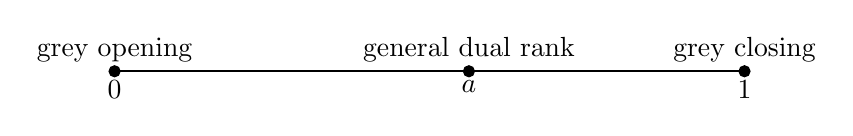
\begin{tikzpicture}
\draw[thick,-] (0,0) -- (8,0);
\draw[fill] (0,0) circle [radius=2pt];
	\node[below] at (0,0) {$0$};
	\node[above] at (0,0) {grey opening};
\draw[fill] (4.5,0) circle [radius=2pt];
	\node[below] at (4.5,0) {$a$};
	\node[above] at (4.5,0) {general dual rank};
\draw[fill] (8,0) circle [radius=2pt];
	\node[below] at (8,0) {$1$};
	\node[above] at (8,0) {grey closing};
\end{tikzpicture}
\end{center}
\subsubsection{Ground extraction}
The dual rank operator or grey opening can also be used to produce a DEM (Digital Elevation Map). This is achieved by taking the $z$ values and applying a dual rank operator to them within an $(x,y)$-window. The idea is that this causes the features of the landscape to be pushed into the ground. The ground gets smoothed -- perhaps too much if this process is carried out too violently -- and the other objects ``melt".
\newpage
\begin{figure}[!h]
  \caption{Road, raw intensity}
  \centering
    \includegraphics[width=0.9\textwidth]{road.png}
    \label{rd}
\end{figure}
\begin{figure}[!h]
  \caption{Road, grey opening intensity}
  \centering
    \includegraphics[width=0.9\textwidth]{roadga.png}
    \label{rdgo}
\end{figure}
\newpage
\newpage
\begin{figure}[!h]
  \caption{Curvature entropy, raw, $k=50$, $\epsilon = 0.75$, $v=2$, $u=0.1$}
  \centering
    \includegraphics[width=0.9\textwidth]{entropyraw.png}
    \label{ent00}
\end{figure}
\begin{figure}[!h]
  \caption{Curvature entropy, dual operator, $k=50$, $\epsilon = 0.75$, $v=2$, $u=0.1$, $a=0.25$}
  \centering
    \includegraphics[width=0.9\textwidth]{entropy25.png}
    \label{ent25}
\end{figure}
\newpage
\begin{figure}[!h]
  \caption{Curvature entropy, dual operator, $k=50$, $\epsilon = 0.75$, $v=2$, $u=0.1$, $a=0.75$}
  \centering
    \includegraphics[width=0.9\textwidth]{entropy75.png}
    \label{ent75}
\end{figure}
\newpage
\section{Generalised approaches}
%We now have a library of signals. The idea is that the number of signals we have should be sufficient to select features from whichever landscape we're studying.
%
%We should begin by updating our language slightly. What we've considered as signals so far are simply new attributes for the points in a point cloud. We'll call these \textbf{DAs (derived attributes)}.
%
%Thus we have a family of DAs, which inhabit a family of data types $S_0,S_1,S_2,\dots$ and we should be able to write down definitions of the different features which we wish to extract, using only these signals (though, we may have to iterate this process). The elementary view of point clouds is of course to think of them as subsets of $\mathbb{R}^3$ (or, technically, $D^3$ where $D$ is the appropriate data type) maybe with other attributes thrown in to accomodate return numbers. However, during processing we think of them as subset of the \textbf{DA space} $$S_0\times S_1\times S_2\times\dots.$$ When we filter points through a range of values for these DAs, we are selecting points which inhabit a hypercube inside DA space. Sometimes we need to iterate the process, producing new signals for the selected points and applying another selection to the new points of signal space.
%
%We can view this subset of signal space as \emph{the signal} for the point cloud. If we have a sufficient family of elementary signals, we should be able to use this signal to map a classification onto our points which fits our purpose. However, we make two general points:
%\begin{itemize}
%\item The relations within DA space which define various objects (vegetation, buildings, etc.) may be too complicated for us to spot. They might not be given by filters (=hypercubes).
%\item We need a method for ``zooming out". All of our methods thus far have been to use local geometric properties. This is clearly insufficient: As humans, we realise what objects are by comparing them to other objects. We can tell the difference between a thin tree branch and a conductor (in a point cloud) because the thin tree branch is surrounded by other things, and the conductor clears some of its path.
%\end{itemize}
%We will begin to discuss a few methods which go tackling these problems. Broadly speaking, we will look at distributions as a method for ``zooming out". Machine learning is a possible route to finding the more complex relations in DA space.
%\subsection{Distributions}
%We will take point clouds which have the DAs already attached to them -- correlation coefficients, eigenvalues, curvature, entropy, etc. The DAs tell us the ``local geometric properties" of points which we just mentioned. For example, a straight line or small cluster of points has a low entropy (a perfectly straight line or point has entropy 0), an evenly spread out plane has entropy $\log_3(2)\approx 0.63$, and an evenly spread out volume has entropy $1$ (here we are discussing curvature entropy). Imperfect objects have values which are distributed about these three numbers -- 0, $0.63$ and $1$. If we begin to look at a window in the point cloud (rather than a single point and its nearest neighbours), we can take the distribution of entropies inside that window (normalised so that we get a probability density function), and we should expect to see a distribution with three modes, if it contains all three types of object. Figure \ref{w1} shows a 3 meter window selected from a the base of the building in Figure \ref{gh} -- it appears to show a greenhouse, the ground, and a wall. Figures \ref{w1ent} and \ref{w1xy} show two attribute distributions for Window 1 in Figure \ref{w1}. As predicted, all three object types are present -- with low entropy points (straight lines and point-likes) only making a small appearence. The overall shape of the entropy plot is trimodal but there are some spikes which we didn't necessarily expect -- perhaps these represent specific objects which we don't immediately notice in the picture. The plot of XY-linear regression in Figure \ref{w1xy} is also broadly what we expected because the picture does contain a lot of non-linear objects but also a small family of straight lines (the windows of the greenhouse) which presumably correspond to the spike at 1. 
%
%These plots are produced by takign the vector corresponding to a \emph{numerical} attribute of points, and producing its histogram. Then the histogram is scaled down so that it becomes a probability density function.
%
%Let's generate some more examples. We will look at a conductor on it's own to demonstate the nature of a fairly pure object rather than a mixed one. Figure \ref{w2} is a 1 meter window containing just conductor from Figure \ref{conductor}. As we can see from Figures \ref{w2ent} and \ref{w2xy}, the entropies all occur near low values and the XY-linear regressions all occur near high values.
%
%Figure \ref{w3} shows a 1 meter window selected from the top of a pylon in Figure \ref{pylon}. This is a more interesting object because it is a confusing mixture of states: It involves two crossed, thick cylindrical objects and some thin wires. We would expect certain parts of it to look locally like a straight line and some parts to look like a plane (the surface of the cylinders) and some parts to look 3D (corners) but not many perfectly voluminous areas. Indeed, the entropy plot in Figure \ref{w3ent} reflects this: There are some but not many low values of Entropy, quite a lot of modes in the immediate values and a sharp drop before we reach the very highest values. The XY-linear regression plot in \ref{w3xy} is similarly chaotic - with a small but not insignificant number of points giving the largest values.
%\newpage
%\begin{figure}[!h]
%  \caption{``Greenhouse"}
%  \centering
%    \includegraphics[width=0.9\textwidth]{GreenHouse.png}
%    \label{gh}
%\end{figure}
%\begin{figure}[!h]
%  \caption{Window 1}
%  \centering
%    \includegraphics[width=0.9\textwidth]{Window1.png}
%    \label{w1}
%\end{figure}
%\newpage
%\begin{figure}[!h]
%  \caption{}
%  \centering
%    \includegraphics[width=0.8\textwidth]{Figure_1Ent.png}
%    \label{w1ent}
%\end{figure}
%\begin{figure}[!h]
%  \caption{}
%  \centering
%    \includegraphics[width=0.8\textwidth]{Figure_1xy.png}
%    \label{w1xy}
%\end{figure}
%\newpage
%\begin{figure}[!h]
%  \caption{}
%  \centering
%    \includegraphics[width=0.8\textwidth]{Cond.png}
%    \label{conductor}
%\end{figure}
%\begin{figure}[!h]
%  \caption{Window 2}
%  \centering
%    \includegraphics[width=0.8\textwidth]{Window2.png}
%    \label{w2}
%\end{figure}
%\newpage
%\begin{figure}[!h]
%  \caption{}
%  \centering
%    \includegraphics[width=0.8\textwidth]{Figure_2Ent.png}
%    \label{w2ent}
%\end{figure}
%\begin{figure}[!h]
%  \caption{}
%  \centering
%    \includegraphics[width=0.8\textwidth]{Figure_2xy.png}
%    \label{w2xy}
%\end{figure}
%\newpage
%\begin{figure}[!h]
%  \caption{}
%  \centering
%    \includegraphics[width=0.8\textwidth]{pylon.png}
%    \label{pylon}
%\end{figure}
%\begin{figure}[!h]
%  \caption{Window 3}
%  \centering
%    \includegraphics[width=0.8\textwidth]{Window3.png}
%    \label{w3}
%\end{figure}
%\newpage
%\begin{figure}[!h]
%  \caption{}
%  \centering
%    \includegraphics[width=0.8\textwidth]{Figure_3Ent.png}
%    \label{w3ent}
%\end{figure}
%\begin{figure}[!h]
%  \caption{}
%  \centering
%    \includegraphics[width=0.8\textwidth]{Figure_3xy.png}
%    \label{w3xy}
%\end{figure}
%\newpage
%\subsection{The Jensen-Shannon Divergence}
%A \textbf{probability $n$-vector} is an array
%\begin{displaymath}
%p=\begin{pmatrix}
%p_0&p_1&p_2&\dots &p_{n-1}
%\end{pmatrix}\in [0,1]^{n}
%\end{displaymath}
%such that $\sum_i p_i=1$. The distributions we have looked at so far are probability vectors: To produce them, we choose a number $n$ of bins which we want to partition our attributes into, count the number of points in each bin, and then calculate the proportion $p_i$ of points occuring in the $i$-th bin.
%
%We would like a method of comparing distributions. Of course, a probability $n$-vector is simply an element of the $(n-1)$-simplex
%\begin{displaymath}
%\Delta^{n-1}=\left\{\begin{pmatrix}
%p_0&p_1&p_2&\dots &p_{n-1}
%\end{pmatrix}\in\mathbb{R}^n:p_i\geqslant 0,\sum_ip_i=1\right\}\subseteq \mathbb{R}^n\text{,}
%\end{displaymath}
%it is tempting to use any of the metrics on $\mathbb{R}^n$ in order to decided what it means for two probability vectors to be ``close". However, these are typically not sufficiently sensitive for the purpose of measuring distributions. For these purposes, we need a new metric. Consider, for example, the vectors 
%\begin{align*}
%p&=\begin{pmatrix}
%0.8& 0.2& 0&0& 0&0& 0& 0&0
%\end{pmatrix}\\
%q&=\begin{pmatrix}
%0.9& 0.1& 0&0& 0&0& 0& 0&0
%\end{pmatrix}
%\\
%r&=\begin{pmatrix}
%0.8&0.1&0&0&0& 0& 0& 0.1&0
%\end{pmatrix}.
%\end{align*}
%In the metric $d$ defined by $d(x,y)=\max_i|x_i-y_i|$, $d(p,q)=0.2=d(p,r)$. However, in the metric $j$ defined by 
%\begin{displaymath}
%j(x,y)=H\left(\frac{1}{2}(x+y)\right)-\frac{1}{2}\left(H(x)+H(y)\right),
%\end{displaymath}
%where $H$ denotes shannon entropy of a probability vector, $j(p,q)\approx 0.020$ and $j(p,r)\approx 0.005$, a completely different answer. We call $j$ the \textbf{Jensen-Shannon divergence}. The spheres in the Jensen-Shannon divergence are of a different shape to those induced by the metrics on $\mathbb{R}^n$, as we see in Figure \ref{jsdballs}. We will use the Jensen-Shannon entropy $j$ instead of any of the metrics inhereted from Euclidean space because the shape of its spheres are much more appropriate for comparing probability distributions.
%\newpage
%\begin{figure}[!h]
%  \caption{Spheres in the Jensen-Shannon metric on $\Delta^2$}
%  \centering
%    \includegraphics[width=0.8\textwidth]{jsdball.png}
%    \label{jsdballs}
%\end{figure}
%\begin{figure}[!h]
%  \caption{}
%  \centering
%    \includegraphics[width=0.8\textwidth]{Figure_3xy.png}
%    \label{w3xy}
%\end{figure}
%\newpage
%\subsection{Signal: An array of histograms}
%Suppose we have a point cloud and we split it into a lattice of bins which are made of cubes of the same size. This will give us a family $C_0,C_1,\dots, C_{m-1}$ of cubes, each of which contains a family of points. Those points will have attributes which are derived in previous steps, e.g. entropy, isotropy, linear angle. 
%
%Now let's suppose we choose a collection of signals. Perhaps we choose entropy and planar angle. We can choose a number of bins $n$ into which we wish to split the values of entropy and planar angle, and hence choosing $n^2$ bins for the combination. Therefore, in each cube $C_i$ we have a probability vector $p$ of length $n^2$ which is actually the histogram for the (entropy, planar angle)-pairs.
%\subsection{Supervised machine learning: training the signal space}
%Suppse we wish to extract a certain feature, e.g. conductors. So far the strategy has been to compute a signal for the point cloud, potentially with some chosen parameters, and find a way of using that signal to protect the desired feature while eliminating others. For example, most conductor points have isometry between 0.57 and 0.65, but many other features do not, so the isometry signal drastically reduces the search for conductors. However, such choosing of parameters is a time-consuming, subjective task, and can be hard to generalise and automate. So, we could skip it, by training the machine to recognise features in signal space. The training process is as follows:
%\begin{list}{$\bullet$}{}
%\item Take a point cloud which is representative of the data we will use. 
%\item Classify it manually.
%\item Compute the signals for the classified point cloud. 
%\item Transform each point in the point cloud into a point $(s_0,s_1,s_2,\dots)$ in signal space. We will call these points \textbf{example points}.
%\end{list}
%Then, in order to classify a new point cloud, we would:
%\begin{list}{$\bullet$}{}
%\item Compute the signals for the new point cloud.
%\item Transform each point in the point cloud into a point in signal space. We will call these points \textbf{test points}.
%\item For each test point, find its nearest example point.
%\item Label each test point with the same classification as its nearest example point, where by ``nearest" we mean according to some metric (possibly Euclidean) in signal space.
%\item Map the labels of the test points onto the classifications in the point cloud, thus outputting a classified point cloud.
%\end{list}
%An interesting side-effect is that there may be relations between different objects of which we were not aware, and in fact it may teach us whether or not our library of signals is sufficient.
\subsection{Neighbourhood definitions}
Let's go back to first principles and explain our process in a more abstract way. When attaching new attributes to the point cloud, we do the following:
\begin{enumerate}
\item Let $C$ be the point cloud, considered as a finite set of points, and let $\mathscr{O}C$ be the set of all ordered subsets of the point cloud. A \textbf{neighbourhood definition} is a function
\begin{displaymath}
\mathscr{N}:C\to\mathscr{O}C
\end{displaymath}
such that $c\in \mathscr{N}c$ for each $c\in C$.
\item We can take the \textbf{covariance matrix} or the \textbf{structure tensor} of any ordered set of points, so we have a function
\begin{displaymath}
\mathrm{cov}:\mathscr{O}C\to \mathrm{Sym}_d(\mathbb{R})
\end{displaymath}
where $d$ is the number of dimensions we consider our points to have (usually $d=3$ or $d=4$) and $\mathrm{Sym}_d(\mathbb{R})$ is the set of $d\times d$ symmetric matrices.
\item Derive the eigenvalues and eigenvectors
\begin{displaymath}
\mathrm{eval}:\mathrm{Sym}_d(\mathbb{R})\to \mathbb{R}^{d}
\end{displaymath}
\begin{displaymath}
\mathrm{evec}:\mathrm{Sym}_d(\mathbb{R})\to \mathbb{R}^{d\times d}.
\end{displaymath}
of the covariance matrix.
\item Further manipulate the eigenvectors and eigenvalues, and combine these steps to obtain functions $C\to\mathbb{R}$.
\end{enumerate}
So far, our neighbourhood definition has been to fix a $k$, find the $k$ nearest neighbours of each point, and reject neighbours too far from the point, as dermined by a fixed radius $\epsilon$. We'll now look at optimising and automating the choice of $k$ on a point-by-point basis, in order to avoid a heuristic approach.

The first method which we will investigate for definining a non-heuristic neighbourhood is to minimise dimensional entropy. For each $k$ we have the neighbourhood definition $\mathscr{N}_k$, which therefore induces, for each point, a dimensional entropy $E_{\mathrm{dim},k}$. Relative to this entropy, we define the \textbf{dimensionally optimal $k$ value} as is done in \cite[Section 6.3]{weinmann}, by
\begin{displaymath}
k_\mathrm{opt,dim}=\underset{k}{\mathrm{argmax}}E_{\mathrm{dim},k}.
\end{displaymath}
Of course, we can't maximise over an unbounded number of values of $k$, and we need to cut computational costs, so we still need to set a parameter $k_\mathrm{max}$ which puts an upper bound on the available values of $k$.

To illustrate the evolution of $E_{\mathrm{dim},k}$ as $k$ varies, we will focus on an arbitrary, 10-point segment of conductor points which are pictured in Figure \lnk{arb}. The selected point's dimensional entropy at different values of $k$ are plotted in \lnk{diment0}, and the corresponding dimension distributions are given in Figures \lnk{entpt2} to \lnk{entpt9}. In particular, the jump in dimensional entropy from $k=4$ to $k=5$ can be seen in the difference between Figures \lnk{entpt4} and \lnk{entpt5}.
\newpage  
\begin{figure}[!h]
  \caption{$k_\mathrm{opt}$, $k_\mathrm{max}=10$.}
  \centering
    \includegraphics[width=0.9\textwidth]{kopt.png}
    \label{kopt}
\end{figure}

\begin{figure}[!h]
  \caption{$k_\mathrm{opt}$, $k_\mathrm{max}=10$.}
  \centering
    \includegraphics[width=0.9\textwidth]{kopt1.png}
    \label{kopt1}
\end{figure}
\newpage
\begin{figure}[!h]
  \caption{10 arbitrary conductor points.}
  \centering
    \includegraphics[width=0.9\textwidth]{arb.png}
    \label{arb}
\end{figure}
\begin{figure}[!h]
  \caption{Point 0, $E_{\mathrm{dim},k}$}
  \centering
    \includegraphics[width=0.9\textwidth]{EntropyPt0.png}
    \label{diment0}
\end{figure}
\newpage
\begin{figure}[!h]
  \caption{Point 0, $k=2$, dimensional states}
  \centering
    \includegraphics[width=0.8\textwidth]{Pt0k2.png}
    \label{entpt2}
\end{figure}
\begin{figure}[!h]
  \caption{Point 0, $k=3$, dimensional states}
  \centering
    \includegraphics[width=0.8\textwidth]{Pt0k3.png}
    \label{entpt3}
\end{figure}
\newpage 
\begin{figure}[!h]
  \caption{Point 0, $k=4$, dimensional states}
  \centering
    \includegraphics[width=0.8\textwidth]{Pt0k4.png}
    \label{entpt4}
\end{figure}
\begin{figure}[!h]
  \caption{Point 0, $k=5$, dimensional states}
  \centering
    \includegraphics[width=0.8\textwidth]{Pt0k5.png}
    \label{entpt5}
\end{figure}
\newpage 
\begin{figure}[!h]
  \caption{Point 0, $k=6$, dimensional states}
  \centering
    \includegraphics[width=0.8\textwidth]{Pt0k6.png}
    \label{entpt6}
\end{figure}
\begin{figure}[!h]
  \caption{Point 0, $k=7$, dimensional states}
  \centering
    \includegraphics[width=0.8\textwidth]{Pt0k7.png}
    \label{entpt7}
\end{figure}
\newpage 
\begin{figure}[!h]
  \caption{Point 0, $k=8$, dimensional states}
  \centering
    \includegraphics[width=0.8\textwidth]{Pt0k8.png}
    \label{entpt8}
\end{figure}
\begin{figure}[!h]
  \caption{Point 0, $k=9$, dimensional states}
  \centering
    \includegraphics[width=0.8\textwidth]{Pt0k9.png}
    \label{entpt9}
\end{figure}
\newpage 
\section{Signals in production}
Signals are highlighted in \sh{this colour}. The greatest risks to genericity are highlighted in \bad{this colour}.
\subsubsection{Production pipeline 22}
We begin with a large LAS file.
\begin{list}{}{}
\item \textbf{JSON000}
\item Extract a tile from the large file using the chosen time interval.
\item \textbf{JSON001}
\item Read in the tile from JSON000.
\item Find the points which have classification other than 10.
\item \textbf{JSON002}
\item Read in the tile from JSON000.
\item Find the points which have classification equal to 10.
\item \textbf{JSON003}
\emph{Aim: Denoise the flightline.}
\item Read in the file produced in JSON002 (i.e. points on the flightline).
\item Copy intensity into intensitySnapshot.
\item \bad{Identify points with intensity in the range $[630,730]$. (Relies on nature of equipment.)}\footnote{This range was chosen from noticing that the points in the central flightline fall within it.}
\item Using a python script which implements the \bad{KD-three algorithm with $k=40$,} for the points with intensity in the range $[630,730]$, replace intensity of each point with the number of neighbours it has within a 1 meter radius, with a maximum of 40 neighbours being recorded. This is, of course, a variant of \hyperref[crapptdens]{\sh{point density.}}
\item Identify points which now have the (replaced) intensity $\geqslant 40$ (i.e. $=40$), within the points which originally had intentsity within $[630,730]$.
\item \bad{Within these points, repeat the process above with $k=80$, and radius 0.25.}
\item Identify points which now have the (replaced) intensity $\geqslant 80$ (i.e. $=80$).
\item Classify the points from the output of JSON041 which do not have an intensity in $[630,730]$ as classification 7. 
\item Classify the points which were originally in $[630,730]$ which now have intensity $<80$ as classification 7.
\item Copy intensitySnapshot into intensity.
\item Write the result as a new file.
\item \textbf{JSON004}
\item Merge the results of JSON001 and JSON003.
\item \textbf{JSON010}
\emph{Aim -- Label silly points as noise}
\item This step classifies points which have logically inconsistent or very unusual attributes as noise, i.e. classification 7 (e.g. below sea-level, negative intensity, high return numbers). 
\item \textbf{JSON020}
\emph{Aim -- Use SMRF to detect ground}
\item Use \hyperref[smrf]{\sh{SMRF (Simple Morphological Filter)}} to identify points which are above ground, with the following \bad{parameters}:
\begin{center}
\begin{verbatim}
"slope": 0.1, 
"cut": 0.0,
"window": 18, 
"cell": 1.0, 
"scalar": 0.5, 
"threshold": 0.5, 
\end{verbatim}
\end{center}
\item \textbf{JSON050}
\emph{Aim -- Give some basic classifications to above ground points before further processing (in which those classifications might be changed)}
\item Classify the above ground points which are not on the flight line (i.e. not userData 10) as classification 4.
\item Classify the above ground points which are on the flight line (userData 10) to classification 10.
\item Classify the above ground points which are on the flight line and have userData 7 to classification 7.
\item Write reclassified data to a new file.
\item \textbf{JSON060}
\emph{Aim -- Set points too far from the flightline to ``noise". Same goal in 061.}
\item Select the non-noise points which are not above ground (classification $\neq 4$).
\item Within those points, select the points which are 100 meters from the flightline.
\item Set the points outside of that 100 meter distance to classification 7.
\item Deselect classification 7 points.
\item \textbf{JSON061}
\item Select the points which are not classification 2 (i.e. non-ground).
\item Within those points, select the points which are 100 meters from the flightline.
\item Set the points outside of that 100 meter distance to classification 7.
\item Select only classification 4 points from those.
\item \textbf{JSON071}
\emph{Aim of next few steps -- Denoise based on relation to nearest neighbours}
\item Among first returns, find the $k$-distance with $k=1$, and set the points with $k$-distance $\leqslant 1$ as classification 7, i.e. noise.
\item Among non-first returns, do the same.
\item Merge the results.
\item \textbf{JSON081}
\item Same as JSON081 and JSON082 in previous production.
\item \textbf{JSON091}
\item Same as JSON090 in previous production.
\item \textbf{JSON100}
\emph{Aim -- Use signals to begin extraction of conductors}
\item Set $Z$ equal to \hyperref[smrf]{\sh{HAG}}. (This step to make sure we can use linear angle to extract conductor.)
\item Compute the following signals and set them to corresponding attributes: XY-linear regression, linear regression, planar regression, eigenvalues 0, 1, 2, point density, rank, curvature, isotropy, entropy, planar angle, linear angle.
\item Select points with the following
\begin{align*}
\text{xy linear regression}&\in[0.8,1]\\
\text{linear regression}&\in [0,1]\\
\text{planar regression}&\in[0,1]\\
\text{eigenvalue 0}&\in[0,0.001]\\
\text{eigenvalue 1}&\in[0,10]\\
\text{eigenvalue 2}&\in[0.003,\infty)\\
\text{rank}&\in\{0,1,2\}\\
\text{curvature}&\in[0,0.0033]\\
\text{isometry}&\in [0.57,0.65]\\
\text{entropy}&\in[0,0.5]\\
\text{planar angle}&\in [0,1]\\
\text{linear angle}&\in [0.5,1]\\
\end{align*}
\item \textbf{JSON 110-01,02,03,04,05,06}
\emph{Aim -- A second pass to clean up the selection, eliminating as much vegatation as possible before hough lines}
\item To speed up the exposition, I will use a notation to describe some of the filtering. For a $k$-distance filter, we have two parameters: A number $k$ and a distance $d$. Then we filter points whose $k$-th nearest is more than $d$ meters away. We apply the following $(k,d)$-pairs: 
\begin{align*}
(1,1)\\(2,2)\\(2,2)\\(1,1)\\(3,2.5)\\(3,2.5)\\(2,2)\\(1,1)\\(4,2.75)\\(3,2.5)\\(2,2)\\(1,1)\\(5,3)\\(5,3)\\(4,2.75)\\(3,2.5)\\(2,2)\\(1,1)
\end{align*}
\item Among those points, cluster (using PDAL) with a tolerance of 2 meters and a minimum number of points of 1.
\item Inside each cluster, take the average return index $(\overline a,\overline b)$ (i.e. return $\overline a/\overline b$).
\item Select points with $\overline a=1$ and $1\leqslant \overline b\leqslant 3$, \emph{and} which are non-last returns.
\item Among the resulting points, cluster using a tolerance of 1 meter and minimum number of points 1.
\item Select points which have at least 3 points in their cluster.
\item With a tolerance of 2 meters, cluster the resulting points.
\item Select points which have at least 6 points in their cluster.
\item With a tolerance of 4 meters, cluster the resulting points.
\item Select points which have at least 10 points in their cluster.
\item Select points with
\begin{align*}
\text{eigenvalue 2}&\in[0.002,\infty)\\
\text{rank}&\in\{1,2\}\\
\text{isometry}&\in [0.001,\infty)\\
\text{entropy}&\in[0.001,\infty)\\
\text{linear angle}&\in [0.7,1]
\end{align*}
\item More more $k$-distance filters -- \emph{identical to above}.
\item More clustering methods with tolerance-minimum pairs given by $(2,10)$, $(3,20)$, $(4,40)$, $(4,80)$.
\item \textbf{JSON111}
\item Copy $Z$ into UserZ and set $Z=\mathrm{HAG}$.
\item \textbf{JSON120,125,130}
\item These have not changed from production 21. The filtered points are given classification 14.
\item \textbf{JSON140}
\item Using the hough lines, find a ``corridor" around the conductors.
\item Select the non-conductor points (classification $\neq 14$).
\item \textbf{JSON141}
\emph{Aim -- Generate signals to select pylons plus some intersecting vegetation}
\item Compute the signals with the following parameters:
\begin{verbatim}
"{\"k\":\"50\",\"radius\":\"0.50\",\"thresh\":\"0.001\",
\"spacetime\":\"True\",\"vspeed\":\"2\",\"decimate\":\"False\",\"u\"
:\"0.1\",\"N\":\"6\"}"
\end{verbatim}
\item In order to begin picking pylons, select points with 
\begin{align*}
\text{planar regression}&\in[0,0.8]\\
\text{rank}&=3\\
\text{eigenvalue 1}&\neq 0\\
\text{curvature}&\in[0,0.2]\\
\text{isometry}&\in [0.6,1]\\
\text{planar angle}\in[0.5,1]\\
\text{linear angle}\in[1,0.5]
\end{align*}
\item\textbf{JSON142}
\item Hough lines to pick pylons. 
\item\textbf{JSON150}
\item Set pylons to classification 13.
\end{list}
\subsubsection{Production pipeline 21}
\begin{itemize}
\item \textbf{JSON000}
\begin{itemize}
\item Extract a tile from the large file using the chosen time interval.
\end{itemize}
\item \textbf{JSON005}
\begin{itemize}
\item Read in tile, adding \hyperref[smrf]{\sh{HAG}} (= height above ground) as an extra dimension.
\item Cut up file into equal time intervals.
\item Write the output.
\end{itemize}
\item \textbf{JSON010}
\begin{itemize}
\item Read in the file.
\item Copy (or, in PDAL language, ``ferry") classification into userData. We do this because we will want to refer to the original classifications later ($1$ is non-flightline, $10$ is flight line), but we want to start changing classifications now.
\item Set points with intensity $<0$ to classification 7 and userData 7.
\item Set points with $Z<0$ (below sea level) to classification 7 and userData 7.
\end{itemize}
\item \textbf{JSON020}
\begin{itemize}
\item Use \hyperref[smrf]{\sh{SMRF (Simple Morphological Filter)}} to identify points which are above ground, with the following \bad{parameters}:
\begin{center}
\begin{verbatim}
"slope": 0.1, 
"cut": 0.0,
"window": 18, 
"cell": 1.0, 
"scalar": 0.5, 
"threshold": 0.5, 
\end{verbatim}
\end{center}
\item \bad{Note that AC thinks the ground routine is unreliable in different contexts.}
\end{itemize}
\item \textbf{JSON030}
\begin{itemize}
\item Classify the above ground points which are not on the flight line (i.e. not userData 10) as classification 4.
\item Classify the above ground points which are on the flight line (userData 10) to classification 10.
\item Classify the above ground points which are on the flight line and have userData 7 to classification 7.
\item Write reclassified data to a new file.
\end{itemize}
\item \textbf{JSON040}
\begin{itemize}
\item Read in the file produced in JSON030.
\item Write a new file containing just classification $\neq 10$ points from that file (i.e. flightline points).
\end{itemize}
\item \textbf{JSON041}
\begin{itemize}
\item Read in the file produced in JSON030.
\item Write a new file containing just classification $= 10$ points from that file (i.e. non-flightline points).
\end{itemize}
\item \textbf{JSON042}
\begin{itemize}
\item Read in the file produced in JSON041 (i.e. points on the flightline).
\item Copy intensity into intensitySnapshot.
\item \bad{Identify points with intensity in the range $[630,730]$. (Relies on nature of equipment.)}\footnote{This range was chosen from noticing that the points in the central flightline fall within it.}
\item Using a python script which implements the \bad{KD-three algorithm with $k=40$,} for the points with intensity in the range $[630,730]$, replace intensity of each point with the number of neighbours it has within a 1 meter radius, with a maximum of 40 neighbours being recorded. This is, of course, a variant of \hyperref[crapptdens]{\sh{point density.}}
\item Identify points which now have the (replaced) intensity $\geqslant 40$ (i.e. $=40$), within the points which originally had intentsity within $[630,730]$.
\item \bad{Within these points, repeat the process above with $k=80$, and radius 0.25.}
\item Identify points which now have the (replaced) intensity $\geqslant 80$ (i.e. $=80$).
\item Classify the points from the output of JSON041 which do not have an intensity in $[630,730]$ as classification 7. 
\item Classify the points which were originally in $[630,730]$ which now have intensity $<80$ as classification 7.
\item Copy intensitySnapshot into intensity.
\item Write the result as a new file.
\end{itemize}
\item \textbf{JSON043}
\begin{itemize}
\item Merge the output from steps 40 and 42.
\end{itemize}
\item \textbf{JSON050}
\begin{itemize}
\item Populate the \hyperref[smrf]{\sh{HAG}} attribute using the appropriate filter.
\item Classify points with $\mathrm{HAG}<-0.25$ as classification 7 (below ground noise).
\item Write the result as a new file.
\end{itemize}
\item \textbf{JSON071}
\begin{itemize}
\item Copy $X$ into KDistance (presumably just to get a new attribute of appropriate length and data type).
\item Set $\mathrm{KDistance} = 0$.
\end{itemize}
\item \textbf{JSON072}
\begin{itemize}
\item Read file with HAG and KDistance.
\item Identify points with classification $\neq 7$. (That is, deselect noise.) 
\begin{center}
\bad{Note that PRD020 says return number $\neq 7$. This is a mistake.}
\end{center}

\item Find the distance to $k$-th nearest neighbour among those pionts using PDAL's kdistance filter, $k=1$. That is, find \hyperref[nnd]{\sh{nearest neighbour distance}}.
\item Note that, in the PDAL documentation we have the following comment:
\begin{center}
\begin{verbatim}
The K-distance filter is deprecated and has been replaced by
`filters.nndistance`_.
\end{verbatim}
\end{center}
\item Merge the classification $\neq 7$ and classification 7 points back together.
\item Write $k$-distance into KDistance.
\end{itemize}
\item \textbf{JSON073}
\begin{itemize}
\item Identify points with Classification $\neq 7$, KDistance $>1$ and return number 1. Give those points classification 7. (Not huge risk here unless coordinates are measured in \bad{different units}.)
\item Merge those points back in and set KDistance = 0 for all points.
\begin{center}
\bad{Note that the same return number/classification mix up happens here, too.}
\end{center}
\end{itemize}
\item \textbf{JSON081}
\begin{itemize}
\item Read file with HAG and KDistance.
\item Identify the points with Classification $\neq 7$, and perform the kdistance filter, $k=3$.
\item Merge with rest of points, writing $k$-distance into KDistance.
\end{itemize}
\item \textbf{JSON082}
\begin{itemize}
\item Identify points with Classification $\neq 7$, \bad{KDistance $>1.2$} and return number 1. Give those points classification 7.
\item Merge those points back in and set KDistance = 0 for all points.
\begin{center}
\bad{Note that the same return number/classification mix up happens here, too.}
\end{center}
\end{itemize}
\item \textbf{JSON090}
\begin{itemize}
\item Identify the returns $1/1$ with classification 4 (above ground) and \bad{intensity $<600$.} Set those points to classification 7.
\item Merge those points back in.
\end{itemize}
\item \textbf{JSON100}
\begin{itemize}
\item Identify points with classification 4 (above ground).
\item For those points, copy classification into USERReturnNumber (just to get an attribute of correct type and length.
\item Set USERReturnNumber = $10a+b$ where $a/b$ is the return index.
\item Identify points with USERReturnNumber = $11,22,33,44,55$. (i.e. last returns, assuming numberOfReturns $<6$).
\begin{center}
\bad{According to AC it's better not to do this.}
\end{center}
\begin{center}
\bad{What follows involves in this JSON heavy choice of parameters. This is risky.}
\end{center}
\item Find \hyperref[roc]{\sh{normal curvature}} with $k=8$. Copy this curvature into lovelyCurves008. (After multiplying by 100 with a python filter.)
\item Find normal curvature with $k=101$. Copy this curvature into lovelyCurves101. (After multiplying by 100 with a python filter.)
\item Copy curvature into lovelyCurves and set $\mathrm{lovelyCurves}=0$.
\item Take $\mathrm{lovelyCurves}=\min(\mathrm{lovelyCurves008},\mathrm{lovelyCurves101})$. (Using a python filter.)
\item Identify points with $\mathrm{lovelyCurves}\leqslant 1$. For these points compute the same $\mathrm{lovelyCurvature}$ as above, but relative only to other points with $\mathrm{lovelyCurves}\leqslant 1$. Repeat this process. And repeat again.
\begin{center}
\bad{I think the curvature on line 173 should have been lovely curvature, to fit this pattern}
\end{center}
\item Identify points with $\mathrm{lovelyCurves}\leqslant 1$. Identify the points among those with \hyperref[evalz]
{\sh{eigenvalue 0}} $\leqslant 0.001$, and repeat this step for a further 7 passes.
\item Write out the result along with HAG.
\end{itemize}
\item \textbf{JSON110}
\begin{itemize}
\item WRITE UP THE CLUSTERING STEPS.
\end{itemize}
\item \textbf{JSON111}
\begin{itemize}
\item Copy $Z$ into $\mathrm{userZ}$.
\item Copy HAG into $Z$.
\item Write out the result.
\end{itemize}
\item \textbf{JSON120}
\begin{itemize}
\item Perform hough3D python filter. The \hyperref[hough]{\sh{hough lines}} are found by the following steps.
\begin{itemize}
\item \bad{Clip $4\leqslant\mathrm{HAG}\leqslant 12$.}
\item Select class 2 (non-ground, non-noise).
\item On $6.4\mathrm{m}\times 6.4\mathrm{m}$ subtiles, compute 3d hough lines (using another python script).
\item \bad{Reject hough lines which are more than 82 degrees from the vertical.}
\item After this we put, around each hough line, two polygons $A\subseteq B$ and reject hough lines which have points in $B-A$. (According to AC there is a \bad{threshold} on $|B-A|$.)
\item All selected lines are then written into a file.
\end{itemize}
\end{itemize}
\item \textbf{JSON125}
\begin{itemize}
\item Read file with HAG and userZ.
\item Perform hough3D2 python filter which is a second pass of hough3D to find some points which were missed. (We seem to be lacking clear knowledge of what this step is doing, precisely.)
\item According to AC there is a \bad{bug} in which hough3D2 overwrites hough3D -- presumably the result is equivalent to just doing JSON120 and not doing JSON 125.
\end{itemize}
\item \textbf{JSON130}
\begin{itemize}
\item Set points on hough lines to classification 14 by using applyHough.
\end{itemize}
\item \textbf{JSON135}
\begin{itemize}
\item Read in file with HAG.
\item Perform the ``virus" filter with 
\begin{center}
\begin{verbatim}
 "pdalargs":"{\"itter\":\"1\",\"class\":\"14\",\"clip\":\"0.25\"}"
\end{verbatim}
\end{center}
The virus tool finds all points within a clip (0.25 in this instance) of a certain class of points (classification 14 here), and sets them to the same classification, and repeats a certain number of times (this time we don't repeat). This causes the chosen classification to leak out a little.
\end{itemize}
\item \textbf{JSON140}
\begin{itemize}
\item Apply the pylon extracting python filter to non-classification 14 points (to preserve the conductor we've already extracted). This tool works similarly to the extraction of conductors: Instead of finding horizontal 3D lines, we find vertical ones \bad{by selecting angles $<5$ degrees from the vertical.} This is similar to using the \hyperref[roc]{\sh{angles}} between $\textbf{v}_0$ and the vertical.
\end{itemize}
\item \textbf{JSON150}
\begin{itemize}
\item Set points on conductors to classification 13 using applyHough.
\end{itemize}
\item \textbf{JSON160}
\begin{itemize}
\item Find all points within a $3\mathrm{m}\times 3\mathrm{m}$ cube of conductor (classification 14) which is not classification 14, 13, 10, 7, or 2. 
\item Set those points to classification 15.
\end{itemize}
\item \textbf{JSON170}
\begin{itemize}
\item \textbf{01} Find all points with classification 13, 14 or 15 (putatively, dangerous vegetation, conductor, and pylons, respectively).
\item \textbf{02} Find all points with classification 15 (putative pylon).
\item \textbf{03} Find all points with classification 14 (putative conductor).
\item \textbf{04} Find all points with classification 13 (putative dangerous vegetation).
\item \textbf{12} 
\begin{itemize}
\item Take the output of 02. Calculate curvature $\times 100$ with $k=101$.
\item By taking at most 251 neighbours of any point which fall within a 1 meter radiues, calculate the local median of each point and set to the new curvature. Then do that again, twice. This is an instance of the \hyperref[dual]{\sh{dual rank operator}}.
\item Find the points with \bad{curvature $>2$,} to be thought of as vegetation. 
\item Find the points with \bad{curvature $\leqslant 2$,} to be thought of as buildings.
\item Reclassify the points with curvature $\leqslant 2$ as classification 6.
\item Merge curvature $>2$ and curvature $\leqslant 2$ back together.
\item Use virus to spread classification 6 by 1 meter. Repeat this with clips of 0.5, 0.25, and again by 0.25.
\end{itemize}
\item \textbf{13} 
\begin{itemize}
\item Find classification 6 points and cluster them with a tolerance of 1 meter and at least 1 point in each cluster, using PDAL's \hyperref[clus]{\sh{clustering filter}}.
\item Copy the clusterIDs into clusterIDCountMax and set clusterIDCountMax = 0.
\item Set clussterIDCountMax at any point to the number of points which share the same cluster ID as that point. Cap that count at 10000.
\item Find points with clusterIDCountMax $<1000$, and reclassify them as classification 4.
\item Merge the classification 15, 6 and 4 back together.) 
\end{itemize}
\item \textbf{14} Merge the result of 13 and 4: The new classification 15, 6, 4 and 13, back together.
\item \textbf{15} Take points with classification 6 (building) and 13 (vegetation), and use the virus tool to with 
\begin{center}
\begin{verbatim}
{\"itter\":\"1\",\"class\":\"6\",\"clip\":\"2.00\"}"
\end{verbatim}
\end{center}
to spread classification 6 points over a 2 meter clip. Repeat this step three times.
\item Merge classification 4, 6, 13 and 15.
\item \textbf{16} Merge the result of \textbf{03} and \textbf{15}.
\item\textbf{17}Among the points with classification 6 or 14, use the virus tool with 
\begin{center}
\begin{verbatim}
"{\"itter\":\"1\",\"class\":\"6\",\"clip\":\"0.5\"}"
\end{verbatim}
\end{center}
Repeat this process. 
\item \textbf{18} Merge the results of \textbf{16} and \textbf{01}.
\end{itemize}
\item \textbf{JSON175}\begin{itemize}
\item Load points with HAG.
\item Sort points according to GPS time, with ascending order.
\item Take classification 15 points and cluster them with a tolerance of 1 meter, using PDAL's cluster filter.
\item Copy cluserID into clusterIDCountMax.
\item Set clusterIDCountMax to the number of points which share the same cluster ID as that point. Cap that count at 10000.
\item Set points with $\mathrm{clusterIDCountMax}<500$ as classification 4.
\item Merge these points back in with other points.
\end{itemize}
\item \textbf{JSON200} Using a python function, select points within a shape file.
\end{itemize}
%\subsection{Deforestation}
%In this section we will discuss a signal which seeks to remove the vegetation from the landscape but keep the conductors. We do this by analysing point densities and return numbers.
%
%To reduce the problem, we could remove the ground. There are various approaches we can take to this, but to keep things simple, to remove the ground we'll just keep points with return number less than the number of returns -- i.e. the \emph{not-last returns}. See Figures \lnk{less}, \lnk{equal}, \lnk{houseless} and \lnk{houseequal} for the impact of this on some sample tiles.
%
%Keeping only the non-last returns in lidar data:
%\begin{itemize}
%\item Keeps some of the pylon.
%\item Keeps almost all of the conductor.
%\item Keeps exterior vegetation.
%\item Loses most of the ground. 
%\item Loses most building.
%\end{itemize}
%
%Keeping only the last returns (which includes returns 1/1) in lidar data:
%\begin{itemize}
%\item Keeps the rest of the pylon.
%\item Keeps barely any of the conductor.
%\item Keeps interior vegetation.
%\item Keeps most of the ground. 
%\item Loses most building.
%\end{itemize}
%
%When a conductor is beneath noise, it behaves more like vegetation and has some higher return numbers, e.g. 2/3, as in Figure \lnk{cablenoise}. For this reason, we must use a point count to determine whether we are looking at a region of vegetation or a region containing conductors.
%
%Taking sufficiently extreme return numbers, e.g. 4/5 extracts only the deepest vegetation - see Figure \lnk{ret45}. We can then take a local point count. These point counts could be used to separate noise from real data.
%
%Figure \lnk{extraction} gives a recipe for finding points belonging to conductors. This could be viewed as a signal: it has an input point cloud and an output point cloud.
%
%Our signal here has two parameters, dictated by choices which are (currently) made by humans. They are the shape and size of our local window -- we will use cylinders with a 10 meter radius, but one could use cuboids. The other parameter is a choice of clip. The python shell below shows this process being carried out, with a clip of $100$. Figures \lnk{lessabove} and \lnk{lesstreesremoved} give a before-and-after shot of this process. As input we use the point cloud pictured in Figure \lnk{realdata}.
%
%Figures \lnk{deforest50} and \lnk{deforest5} show the effects of dropping the clip. If we also decreased the radius, our selection would hopefully be better and we wouldn't select away pieces of tree and eventually we could find a ``sweat spot" where we chose the radius (or window shape in general) and a clip such that we do not remove anything but vegetation.
%
%\begin{lstlisting}
%>>> import numpy, laspy
%>>> less = laspy.file.File("NonLastReturn.las", mode = "r")
%>>> ptct = laspy.file.File("RealDataPtCount.las", mode = "r")
%>>> clip = 100
%>>> indices = ptct.intensity>clip
%>>> mask = less.intensity != less.intensity
%>>> xs = ptct.x[indices]
%>>> ys = ptct.y[indices]
%>>> N = sum(indices)
%>>> for index in range(N):
%...     condition = (less.x-xs[index])**2+(less.y-ys[index])**2<10**2
%...     mask = numpy.logical_or(mask,condition)
%... 
%>>> outFile = laspy.file.File("NonLastReturnDeforestation.las", mode = "w", header = less.header)
%>>> outFile.points = less.points[numpy.logical_not(mask)]
%\end{lstlisting}
%
%In reality, we should first denoise before doing this, and our clip could then be set to $1$, so that we are simply going to remove points which are within the same local window of a return 4/5. To denoise, we could use nearest neighbour distances. 
%
%\newpage 
%\begin{figure}[!h]
%  \caption{Extracting conductors}
%  \centering
%    \includegraphics[width=0.9\textwidth]{Extraction.png}
%    \label{extraction}
%\end{figure}
%\newpage
%\begin{figure}[!h]
%  \caption{Return number $<$ Number of returns}
%  \centering
%    \includegraphics[width=0.9\textwidth]{less.png}
%    \label{less}
%\end{figure}
%\begin{figure}[!h]
%  \caption{Return number $=$ Number of returns}
%  \centering
%    \includegraphics[width=0.9\textwidth]{equal.png}
%    \label{equal}
%\end{figure}
%\newpage
%\begin{figure}[!h]
%  \caption{Return number $<$ Number of returns}
%  \centering
%    \includegraphics[width=0.9\textwidth]{houseless.png}
%    \label{houseless}
%\end{figure}
%\begin{figure}[!h]
%  \caption{Return number $=$ Number of returns}
%  \centering
%    \includegraphics[width=0.9\textwidth]{houseequal.png}
%    \label{houseequal}
%\end{figure}
%\newpage
%\begin{figure}[!h]
%  \caption{Cables exhibit returns 2/3 when beneath noise}
%  \centering
%    \includegraphics[width=0.9\textwidth]{cableundernoise.png}
%    \label{cablenoise}
%\end{figure}
%\begin{figure}[!h]
%  \caption{Point cloud used for point counts}
%  \centering
%    \includegraphics[width=0.9\textwidth]{realdataclipped.png}
%    \label{realdata}
%\end{figure}
%\newpage
%\begin{figure}[!h]
%  \caption{Returns 4/5}
%  \centering
%    \includegraphics[width=0.9\textwidth]{ret45.png}
%    \label{ret45}
%\end{figure}
%\begin{figure}[!h]
%  \caption{Point count in returns 4/5}
%  \centering
%    \includegraphics[width=0.9\textwidth]{ret45pt.png}
%    \label{ret45pt}
%\end{figure}
%\newpage
%\begin{figure}[!h]
%  \caption{Return number $<$ Number of  returns, from above}
%  \centering
%    \includegraphics[width=0.9\textwidth]{lessabove.png}
%    \label{lessabove}
%\end{figure}
%\begin{figure}[!h]
%  \caption{Result of process to remove trees, $\epsilon =10$, $\mathrm{clip}=100$}
%  \centering
%    \includegraphics[width=0.9\textwidth]{lesstreesremovedradius10clip100.png}
%    \label{lesstreesremoved}
%\end{figure}
%\newpage
%\begin{figure}[!h]
%  \caption{Result of process to remove trees, $\epsilon =10$, $\mathrm{clip}=50$}
%  \centering
%    \includegraphics[width=0.9\textwidth]{lesstreesremovedradius10clip50.png}
%    \label{deforest50}
%\end{figure}
%\begin{figure}[!h]
%  \caption{Result of process to remove trees, $\epsilon =10$, $\mathrm{clip}=5$}
%  \centering
%    \includegraphics[width=0.9\textwidth]{lesstreesremovedradius10clip5.png}
%    \label{deforest5}
%\end{figure}
%\newpage
%\subsection{The center of intensity vs center of unity}
%If we were to compute the center of mass of a body with uniform density, we would obtain the mean position of points within that body. This is obvious, but the converse says that if the center of mass is not the mean position then the body in question is inhomogeneous in density. We now base a signal on that reasoning.
%
%Let points be given with position vectors $\textbf{r}_1,\textbf{r}_2,\dots,\textbf{r}_n$ and corresponding intensities $I_1,I_2,\dots,I_n$. Their \textbf{center of intensity} is 
%\begin{displaymath}
%\mathrm{CoI}={\sum^n_{i=1}I_i\textbf{r}_i}\left/{\sum^n_{i=1}I_i}\right.
%\end{displaymath}
%and their \textbf{center of unity} is
%\begin{displaymath}
%\mathrm{CoU}=\left.\sum^n_{i=1}\textbf{r}_i\right/ n.
%\end{displaymath}
%When we calculate the center of intensity for lidar data, we must be careful, because it is a 16-bit integer. We will change the intensities to floats.
%
%If the distance between these points,
%\begin{displaymath}
%\lVert \mathrm{CoI}-\mathrm{CoU}\rVert,
%\end{displaymath}
%is large then this points to an ``uneven variation" of intensity. For the test area given in Figure \lnk{realdata}, these two centers are extremely close, as shown below.
%\begin{lstlisting}
%>>> import numpy, laspy
%>>> inFile = laspy.file.File("RealDataClipped.las", mode = "r")
%>>> xs = inFile.x
%>>> ys = inFile.y
%>>> zs = inFile.z
%>>> CoM = numpy.array([numpy.mean(xs),numpy.mean(ys),numpy.mean(zs)])
%>>> CoI = numpy.array([numpy.mean(Is*xs)/numpy.mean(Is), numpy.mean(Is*ys)/numpy.mean(Is), numpy.mean(Is*zs)/numpy.mean(Is)])
%>>> numpy.sqrt(sum((CoI - CoM)**2))
%6.988626965596175
%\end{lstlisting}
%We should expect this, as a large chunk of rural landscape is broadly homogeneous. However, on a smaller scale we don't expect such variation, and by taking $\lVert \mathrm{CoI}-\mathrm{CoU}\rVert$ inside a small area, i.e., our balls $B_\epsilon(x,y,z)$, we produce a signal that measures the amount of change in the type of material appearing in that ball. Otherwise, if the contents of our ball are homogeneous, we don't expect this signal attain a large value there (relative to $\epsilon$). 
%
%In Figure \lnk{coicom}, which is plotted with radius $\epsilon =1$, we observe the following:
%\begin{itemize}
%\item The walls of a house yield low values for this signal, but the corners offer high values. 
%\item Vegetation yields low values in its interior and high values on its exterior.
%\item Ground yields low values.
%\item Conductors yield low values until they meet pylons.
%\end{itemize}
%Figures \lnk{bus} and \lnk{buscoi} emphasise the behaviour of this signal -- its value jumps up whenever the intensity of the surrounding area changes.
%\newpage
%\begin{figure}[!h]
%  \caption{Three sample data sets}
%  \centering
%    \includegraphics[width=0.9\textwidth]{housecoicom.png}
%    \label{wonder}
%\end{figure}
%\begin{figure}[!h]
%  \caption{CoI vs CoM -- red areas have a difference of 10cm+}
%  \centering
%    \includegraphics[width=0.9\textwidth]{coicom.png}
%    \label{coicom}
%\end{figure}
%\newpage
%\begin{figure}[!h]
%  \caption{Markings on the road}
%  \centering
%    \includegraphics[width=0.9\textwidth]{busstoptile.png}
%    \label{bus}
%\end{figure}
%\begin{figure}[!h]
%  \caption{CoI vs CoU for markings on road}
%  \centering
%    \includegraphics[width=0.9\textwidth]{BusStopCenters.png}
%    \label{buscoi}
%\end{figure}
%\newpage
%\newpage
%\subsection{Intensity histograms}
%A simple 1-dimensional signal is the intensity histogram for a point cloud. For the point cloud in Figure \lnk{thirteen}, we can make a histogram of the intensities in a python shell as follows.
%\begin{lstlisting}
%>>> import matplotlib.pyplot as plt
%>>> import numpy, laspy
%>>> inFile = laspy.file.File("RealDataClipped.las", mode = "r")
%>>> N = len(numpy.unique(inFile.intensity))
%>>> plt.hist(inFile.intensity, bins = N)
%(array([ 6., 10.,  9., ...,  0.,  0.,  1.]), array([  25.        ,   25.99977528
%,   26.99955056, ..., 4472.00044944,
%       4473.00022472, 4474.        ]), <a list of 4450 Patch objects>)
%>>> plt.title("Intensity Histogram")
%Text(0.5, 1.0, 'Intensity Histogram')
%>>> plt.show()
%\end{lstlisting}
%The resulting plot is shown in Figure \lnk{inthist}. The same plot for the point cloud of a single tree, with the ground removed, is shown in Figure \lnk{inthisttree}. In the tree's histogram, we can see a tall, wide peak which is mostly given by the tree's leaves. The smaller, narrower peak is given by the tree's trunk. 
%
%It's easy to guess where the features in the tree's histogram come from. It's not so easy to tidy up the histogram for the large tile given in Figure \lnk{inthist}.
%\newpage 
%\begin{figure}[!h]
%  \caption{An intensity histogram of a large tile}
%  \centering
%    \includegraphics[width=1\textwidth]{IntensityHistogram.png}
%    \label{inthist}
%\end{figure}
%\begin{figure}[!h]
%  \caption{An intensity histogram of a tree}
%  \centering
%    \includegraphics[width=1\textwidth]{TreeIntsHist.png}
%    \label{inthisttree}
%\end{figure}
%\newpage
%\subsection{Minimum and maximum values}
%\subsection{Distance to next return number}
\newpage
\begin{thebibliography}{99}
\bibitem{poole} David Poole, \emph{Linear Algebra: A Modern Introduction.} Thomson Brooks/Cole, 2006.
\bibitem{eckstein} W. Eckstein and O. Munkelt, \emph{Extracting objects from digital terrain
models.} Proceedings of the International Society for Optical Engineering: Remote Sensing
and Reconstruction for Three-Dimensional Objects and Scenes, 1995.
\bibitem{weinmann} Martin Weinmann, \emph{Reconstruction and Analysis
of 3D Scenes}. Springer International Publishing Switzerland, 2016.
\end{thebibliography}
\end{document} 
